\chapter{Introduction to microresonator-based frequency combs}
 \label{chap:microresonators}

 
 This chapter introduces the basic physics of optical frequency-comb generation in Kerr-nonlinear microring resonators, with a particular emphasis on providing context for the results described in the subsequent chapters. This field emerged in 2007 with the first report of comb generation in silica microtoroids \cite{DelHaye2007}, and continues to evolve rapidly. There are facets to the field that are not discussed here; we note that a number of papers that review this topic have been published, each of which provides a unique perspective \cite{Kippenberg2011,Savchenkov2016,Chembo2016a,Pasquazi2018}. The combs generated in Kerr-nonlinear ring resonators, excluding those generated in definitively `macro' fiber loops, have generally been called microcombs, despite the fact that some of the resonators used to generate them have dimensions on the order of several millimeters. Microcombs are an attractive technology because of their high repetition rates and small footprints, especially relative to modelocked-laser-based combs, which make them promising candidates for inclusion in integrated photonics systems. Microcomb generation has been reported in a variety of platforms, including the aforementioned silica microtoroids, silica wedge \cite{Lee2012,Yi2015} and rod \cite{DelHaye2013} resonators, crystalline magnesium-fluoride \cite{Liang2011} and calcium-fluoride \cite{Savchenkov2008} resonators, and silicon-nitride waveguide resonators \cite{Okawachi2011,Moss2013}, which have the advantage of being immediately amenable to photonic integration.
 
 For simplicity, and following the terminology of the field, we will refer to broadband optical spectra generated through frequency conversion in Kerr-nonlinear microring resonators as `Kerr combs,' even when the output is not strictly a coherent frequency comb. Finally, we note that although researchers have so far focused on Kerr-comb generation with the ring geometry, is also possible to generate Kerr combs in a Kerr-nonlinear Fabry-Perot (FP) cavity, as has been demonstrated in two experiments \cite{Braje2009,Obrzud2017}. Theoretical investigations of Kerr-comb generation with the FP geometry are presented in Chapter \ref{chap:FPLLE}.
 

 
 \section{Optical microring resonators} \label{sec:OMRR}
An optical microring resonator guides light for many round trips around a closed path in a dielectric medium by total internal reflection. The principle is the same as the guiding of light in an optical fiber, and indeed a `macroring' resonator can be constructed from a loop of fiber, using a fiber-optic coupler with a small coupling ratio as an input/output port. Microring resonators can be constructed by looping an optical waveguide back on itself, in which case the resonator provides index contrast and light confinement over a full 360\textsuperscript{o} of the modal cross-section. Alternatively, resonators can be realized with geometries that lack an inner radius dimension and therefore provide less spatial confinement. In this case they can host `whispering-gallery modes,'\footnote{In some sources the terminology `whispering-gallery mode resonator' has been applied more generally, but the analogy to the acoustic case seems most appropriate for resonators in which index contrast is not provided over a full 360\textsuperscript{o} of the modal cross-section. Otherwise it is unclear what makes a WGM resonator different from a fiber loop, which in the limit of large radius obviously does not host whispering-gallery modes. This issue of terminology is discussed in Ref. \cite{Ilchenko2006}.} so-called due to their similarity with the acoustic `whispering-gallery' waves that permit a listener on one side of St. Paul's cathedral (for example) to hear whispers uttered by a speaker on the other side of the cathedral. A schematic depiction of the basic components of a typical microring-resonator experiment is shown in Fig. \ref{fig:microringresonator}. Optical microring resonators have a host of characteristics that make them useful for photonics applications in general and for nonlinear optics in particular; these include the ease with which they can be integrated and the ability to tailor the spectral distribution of guided modes through careful resonator design, as well as the ultra-high quality factors that have been demonstrated ($\geq$several hundred million). The resonator quality factor $Q$ is defined as $Q=\omega_0 \tau_{ph}=\nu_0/\Delta\nu$, where $\omega_0=2\pi\nu_0$ is the optical angular frequency, $\tau_{ph}$ is the photon lifetime, and $\Delta\nu$ is the resonance linewidth. The $Q$ can be interpreted literally as the optical phase which is traversed by the carrier wave during the photon lifetime and is a useful figure of merit for nonlinear optics.

\begin{figure}[htpb]
	\begin{center}
		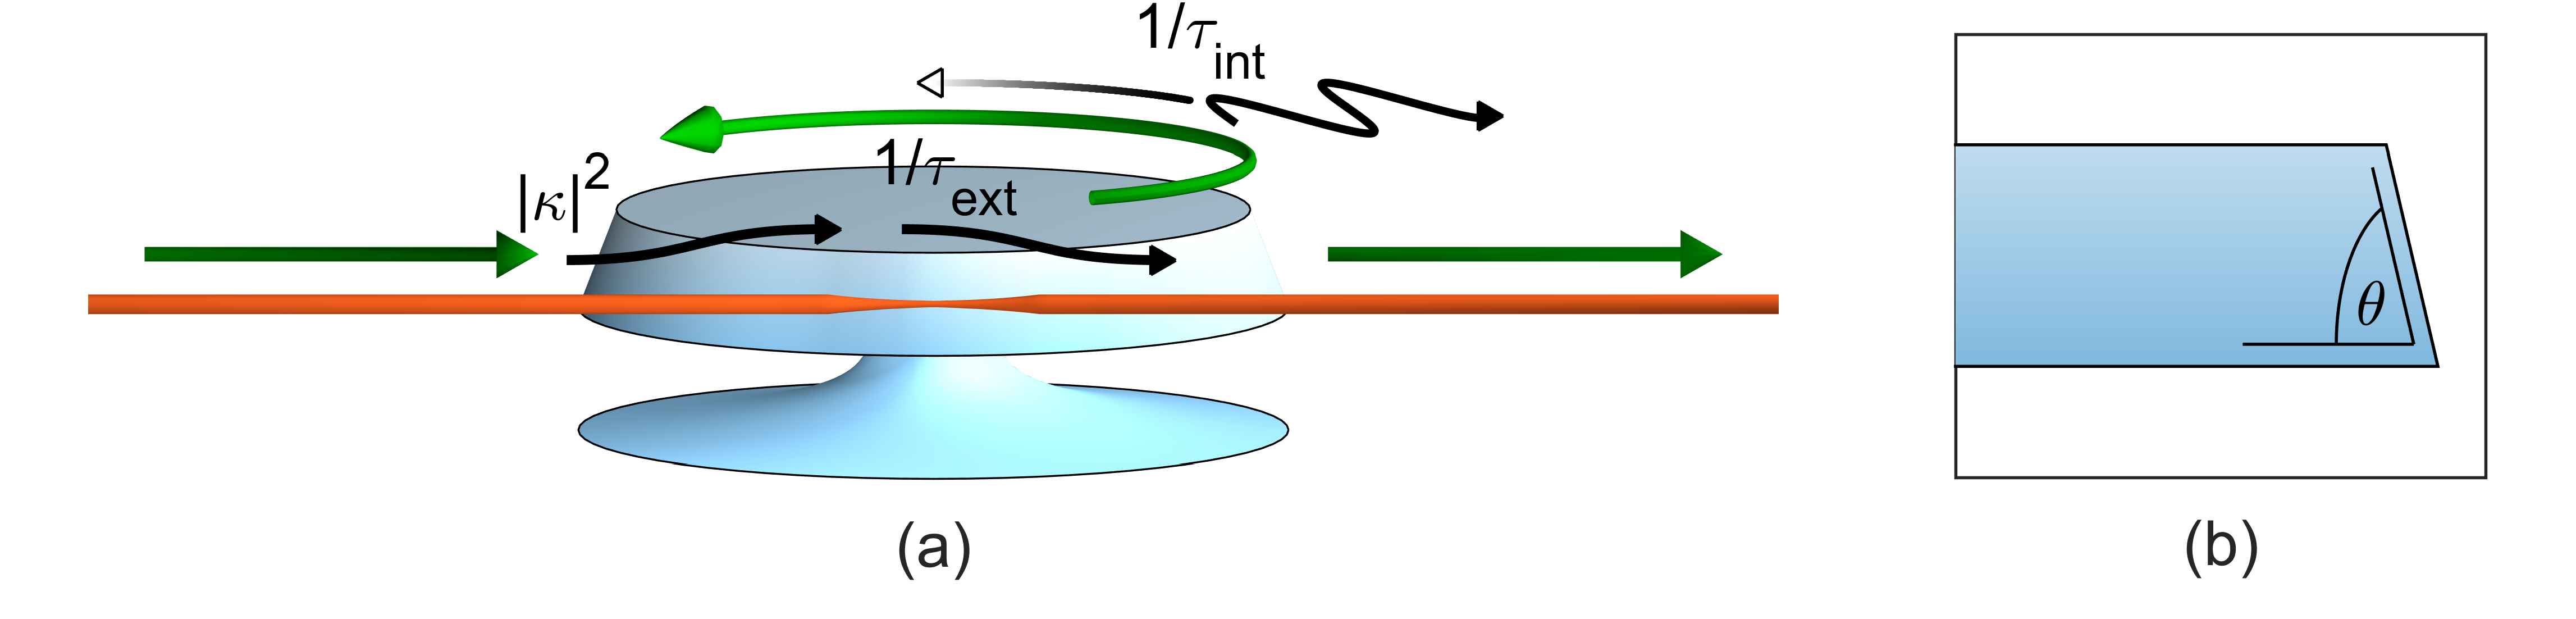
\includegraphics{\FigPath/Figures/Microresonators/MRmicroringresonatorv2.png}
	\end{center}
	\caption[Optical microdisk resonator]{\textbf{Optical microdisk resonator.} (a) An optical microring resonator with the disk geometry as described in Ref. \cite{Lee2012}, operated in a through-coupled configuration. Light (green) is evanescently coupled into and out of the resonator through a tapered optical fiber, shown in orange, which contacts the resonator near the fiber's point of smallest diameter. Light circulates in whispering-gallery modes concentric to the resonator's circumference. The black labels indicate the coupling and loss rates discussed in Sec. \ref{sec:resenhancement}: $|\kappa|^2$ is the rate at which incoming photons are coupled into the resonator, $1/\tau_{ext}$ is the rate at which circulating photons are coupling into the waveguide, and $1/\tau_{int}$ is the intrinsic loss rate. Here contributions to $1/\tau_{int}$ from absorption and radiative losses are depicted. (b) The wedge angle $\theta$ can be adjusted to control the geometric dispersion of the propagating whispering-gallery modes as described in Ref. \cite{Yang2016}, as $\theta$ dictates, for example, the extent to which larger (longer-wavelength) modes are confined further from the circumference of the wedge. }
	
	\label{fig:microringresonator}
\end{figure} 


A microring resonator supports propagating guided modes of electromagnetic radiation with (vacuum) wavelengths that evenly divide the optical round-trip path length: $\lambda_m=n_{eff}(\lambda_m)L/m$, with associated resonance frequencies $\nu_m=c/\lambda_m=mc/n_{eff}(\nu_m)L$. This leads to constructive interference from round trip to round trip. Here $m$ is the azimuthal mode number and the quantity $Ln_{eff}(\lambda_m)$ is the optical round-trip path length of the mode, where $n_{eff}(\lambda_m)$ defines an effective index of refraction related to the mode's propagation constant $\beta_{prop}(\omega)$ via $\beta_{prop}(\omega)=n_{eff}(\omega)\omega/c$ (see e.g. Refs. \cite{Agrawal2007,Calvo2007}; we use the subscript $prop$ to remove ambiguities arising from the standard use of the symbol $\beta$ for multiple quantities). The free-spectral range $f_{FSR}$ of a resonator is the \textit{local} frequency spacing between modes, calculated via:
\begin{align}
	f_{FSR}&\approx \frac{\nu_{m+1}-\nu_{m-1}}{2}\\
	&=\frac{\partial\nu_m}{\partial m},\\
	&=\frac{c}{n_{eff}(\nu)L}-\frac{mc}{n_{eff}^2(\nu)L}\frac{\partial n_{eff}}{\partial \nu}\frac{\partial \nu}{\partial m},
	\end{align}
	so that, rearranging, we obtain:
	\begin{equation}
	f_{FSR}=\frac{c/L}{\left(n_{eff}+\nu\frac{\partial n_{eff}}{\partial \nu}\right)}=\frac{c}{n_g L}=1/T_{RT},
\end{equation}
	where $n_g=n_{eff}+\nu\frac{\partial n_{eff}}{\partial \nu}$ is the group velocity of the mode and $T_{RT}$ is the mode's round-trip time. The effective index $n_{eff}$ is frequency dependent due to both intrinsic material dispersion and geometric dispersion, where the latter results for example from different sampling of material properties for different wavelength-dependent mode areas. A frequency-dependent $n_{eff}$ leads to a non-uniform spacing in the cavity modes in frequency despite the linearity of $\nu_m$ in $m$; equivalently this results in a frequency dependence of $n_g$ and $f_{FSR}$.
	
Depending on the design, microring resonators can support many transverse mode profiles, or just one. The former is typical of whispering-gallery-mode resonators that lack an inner radius, such as the wedge resonator shown in Fig. \ref{fig:microringresonator} or free-standing silica microrod resonators \cite{DelHaye2013}; the latter can be readily achieved using chip-integrated single-mode photonic waveguides. For a given resonator geometry, to calculate the frequency-dependent effective index $n_{eff}(\nu)$, thereby enabling calculation of the resonance frequencies and wavelengths, one must solve Maxwell's equations for the resonator geometry. Except in special cases of high symmetry (e.g. a sphere \cite{Oraevsky2002}), this is typically done numerically using finite-element modeling tools like COMSOL. The modes of an optical resonator, both within a mode family defined by a transverse mode profile (such that they differ only by azimuthal mode number $m$) and between mode families, must be orthogonal \cite{Haus1984}, with no linear coupling between them.

\subsection{Resonant enhancement in a microring resonator} \label{sec:resenhancement}
 The lifetime $\tau_{ph}$ of circulating photons in a resonator is fundamental to its fitness for applications. Generally, two processes lead to the loss of circulating photons: intrinsic dissipation that occurs at a rate $1/\tau_{int}$ and out-coupling to an external waveguide that occurs at a rate $1/\tau_{ext}$, leading to a total loss rate of $\tau_{ph}^{-1}=\tau_{ext}^{-1}+\tau_{int}^{-1}$. To understand the quantitative role of these parameters, we consider a cavity mode of frequency $\omega_0$ and amplitude $a$ (normalized such that $|a|^2=N$, the number of circulating photons) driven by a pump field with frequency $\wpl$ and rotating amplitude $s\propto\exp(i\wpl t)$ (normalized such that $|s|^2=S$, the rate at which photons in the coupling waveguide pass the coupling port) that is in-coupled with strength $\kappa$. The equation of motion for such a system is \cite{Haus1984}:
 \begin{equation}
 \frac{d a}{d t}=i\omega_0 a-\left(\frac{1}{2\tau_{int}}+\frac{1}{2\tau_{ext}}\right)a+\kappa s, \label{eq:coupledmotion}
 \end{equation}
 and the rates that determine the evolution of $a$ are shown schematically in Fig. \ref{fig:microringresonator}. We can immediately solve this equation by assuming that $a\propto\exp(i\wpl t)$, and we obtain:
 \begin{equation}
 a=\frac{\kappa s}{\left(\frac{1}{2\tau_{int}}+\frac{1}{2\tau_{ext}}\right)+i(\wpl-\omega_0)}. \label{eq:coupledsoln}
 \end{equation}
 
The coupling strength $\kappa$ into the waveguide and the out-coupling rate $1/\tau_{ext}$ are related by $|\kappa|^2=1/\tau_{ext}$; one can arrive at this conclusion by considering the special case $1/\tau_{int}=0$ and exploiting the time-reversal symmetry of the system under this condition \cite{Haus1984}. By squaring Eq. \ref{eq:coupledsoln} and inserting this relationship between $\kappa$ and $\tau_{ext}$, we find:
% 
% To extract anything further from this equation, we must derive a relationship between $\tau_{ext}$ and $\kappa$, which so far are not related. To do this, we exploit the time-reversal symmetry that is inherent in this system when there is no dissipation, that is, when $1/\tau_{int}=0$. In the case of only an initial excitation $N_0$ decaying into the waveguide with the driving term $s$ set to zero, we have $N=N_0e^{-t/\tau_{ext}}$. In this case, energy conservation guarantees that the rate $S_{out}$ at which photons propagate away from the resonator in the waveguide is $S_{out}=-dN/dt=N_0e^{-t/\tau_{ext}}/\tau_{ext}$; we therefore have $S_{out}=N/\tau_{ext}$. In the time-reversed system with $t\rightarrow-t$, this amplitude $S_{out}$ describes the rate of pumping: the cavity is resonantly driven with increasing power $S=S_{out}(-t)=N_0e^{t/\tau_{ext}}/\tau_{ext}$. In this case the frequency of the driving field $s$ can be written $\omega_0-i/2\tau_{ext}$. Inserting this frequency into Eq. \ref{eq:coupledsoln} gives the equations
% \begin{equation}
%  a=\kappa s \tau_{ext}
%  \end{equation}
%  and
%  \begin{equation}
%   N=|\kappa|^2 S \tau_{ext}^2.
%   \end{equation}
%   By comparing the relationships between $S_{out}$ and $N$ for the forward-evolving system and $S$ and $N$ for the backward-evolving system, we arrive at the relationship $|\kappa|^2=1/\tau_{ext}$. We can return to the case including dissipation and insert this expression for $\kappa$ into Eq. \ref{eq:coupledsoln}, which can then be squared to obtain:
   \begin{equation}
   N=\frac{\Delta\omega_{ext}S}{\Delta\omega_{tot}^2/4+(\wpl-\omega_0)^2}, \label{eq:resenhancement}
   \end{equation}
   where we have defined the rates $\Delta\omega_{ext}=1/\tau_{ext}$, $\Delta\omega_{int}=1/\tau_{int}$, and $\Delta\omega_{tot}=\Delta\omega_{ext}+\Delta\omega_{int}$. Two important observations can be drawn from Eq. \ref{eq:resenhancement}: First, the cavity response is Lorentzian with a full-width at half-maximum (FWHM) linewidth that is related to the photon lifetime via $\tau_{ph}=1/\Delta\omega_{tot}$, and second, on resonance the number of circulating photons is related to the input rate by the factor $\Delta\omega_{ext}/\Delta\omega_{tot}^2$. The resonant enhancement in the cavity can be calculated from this equation by considering the circulating power $P=N\hbar\omega_p/T_{RT}$ on resonance (when $\omega_p=\omega_0$):
   \begin{align}
   P=&\frac{4\Delta\omega_{ext}P_{in}/T_{RT}}{\Delta\omega_{tot}^2}\\
   =&\frac{2 }{\pi}P_{in}\eta\mathcal{F},
   \end{align}
   where $\mathcal{F}=2\pi\tau_{ph}/T_{RT}=f_{FSR}/\Delta\nu$ is the resonator finesse, $\eta=\Delta\omega_{ext}/\Delta\omega_{tot}$ is the coupling ratio, and $P_{in}=\hbar\omega_p S$ is the power in the waveguide. Thus, the circulating power is approximately a factor $\mathcal{F}$ greater than the input power. The combination of this resonant enhancement and a small cavity mode volume enables very large circulating optical intensities in high finesse resonators, which is important for the application of microresonators in nonlinear optics. 
   
%   
%   
%   Two commonly used practical quantities are linked to the photon lifetime: the resonator finesse $\mathcal{F}=2\pi\tau_{ph}/T_{RT}$, which for a ring resonator can be interpreted literally as the azimuthal resonator angle traced out by a typical photon over its lifetime; and the resonator quality factor $Q=\omega_c \tau_{ph}$, the phase over which the optical field evolves during the photon lifetime. Using the relationship $\tau_{ph}=1/\Delta\omega_{tot}$, the finesse and quality factor can be rewritten as simple ratios of the relevant frequencies: $\mathcal{F}=f_{FSR}/\Delta\nu$; $Q=\nu_c/\Delta\nu$, where $\Delta\nu=\Delta\omega_{tot}/2\pi$.
   
   
  
 
 
% 
% 
% Energy conservation ensures that the rate at which photons propagate away from the resonator in the coupling waveguide is $|s|^2=S=-dN/d t=\frac{N_0}{\tau_{ext}}\exp(-t/\tau_{ext})$. We can consider the time-reversed system in which the input increases in magnitude as $S=\frac{N_0}{\tau_{ext}}\exp(t/\tau_{ext})$ and is resonant with the cavity mode. In this case, the frequency of the drive $s$ is $\omega_s=\omega_0-i/2\tau_{ext}$. Inserting this frequency into Eq. \ref{eq:coupledsoln} for the case of $\Delta\omega_{int}=0$ yields:
% However, for the system without time reversal we have $N=N_0\exp(-t/\tau_{ext})$, $S=\frac{N_0}{\tau_{ext}}\exp(-t/\tau_{ext})$, so that $N=\tau_{ext} S$. By inserting this into the previous equation, we obtain . 
% This is quantified by the basic relation for the number of circulating photons $N(t)=N_oe^{-t/\tau_{ph}}$ in the presence of solely linear loss, which defines the photon lifetime $\tau_{ph}$. 
%
%\begin{equation}
%\mathcal{F}\{E\}(\omega)\propto\int_0^\infty dt\, e^{-\left(\frac{1}{2\tau_{ph}}+i(\omega_c-\omega)\right)t},
%\end{equation}
%which immediately yields the Lorentzian lineshape
%\begin{equation}
%|\mathcal{F}\{E\}|^2\propto\frac{1}{(\omega-\omega_c)^2+\frac{1}{4\tau_{ph}^2}}, \label{eq:lorentzian}
%\end{equation}
%with FWHM linewidth $\Delta\omega=1/\tau_{ph}$. With this relationship, 
%
%The utility of a resonator with long photon lifetime is illustrated by calculating the steady-state number of circulating photons $N$ in a system including a driving term $S$ denoting the rate at which photons are added\cite{Haus1984}. Working in the field quantities $a$ ($|a|^2=N$) and $s$ ($|s|^2=S$), the equation of motion for such a system is: 
%
%The terms in this equation represent the rotation of the field at the mode's frequency $\omega_0$, the strength $\kappa$ of coupling from the input waveguide to the resonator, and the intrinsic and extrinsic (power) loss timescales $\tau_{int}=1/\Delta\omega_{int}$ and $\tau_{ext}=1/\Delta\omega_{ext}$ due to loss and outcoupling. If the drive has frequency $\omega_s$, 
%
%The rates $\Delta\omega_{ext}$ and $\kappa$ are not \textit{a priori} related, but we can derive the relationship between them by exploiting the time-reversal symmetry of systems without dissipation. For the case of no pumping ($s=0$) and no losses ($\Delta\omega_{int}=0$), we have 
%\begin{align}
%\frac{d a}{dt}&=i\omega_0 a-\frac{a}{2\tau_{ext}},\\
%\Rightarrow &a=a_0\exp(i\omega_0 t-t/2\tau_{ext}), \\
%&N=N_0\exp(-t/\tau_{ext}).
%\end{align}





%For the case without dissipation, then, we know that $N=S\tau_ext$, which is the solution of the rate equation
%\begin{equation}
%\frac{dN}{dt}=-N
%\end{equation}
%
%We can now derive a rate equation describing $N(t)$ from Eq. \ref{eq:coupledmotion}:
%\begin{align}
%\frac{dN}{dt}=\frac{d|a|^2}{dt}=a^*\frac{da}{dt}+a\frac{da^*}{dt}
%\end{align}





%Thus the steady-state number of circulating photons and therefore the intensity is larger than the input rate by a factor of the photon lifetime. Of course a more complete calculation including effects such as outcoupling at the coupler (with a rate related to the driving term $A$) could be performed, but this simple calculation captures the essence of the importance of photon lifetime $\tau_{ph}$. \todo{I am not sure whether this captures the scaling that I want to indicate}

\subsection{Thermal effects in microresonators} \label{sec:thermaleffects}

%In a typical microresonator frequency-comb experiment, a frequency-tunable pump laser is coupled evanescently into and out of the resonator using a tapered optical fiber (for e.g. free-standing silica disc resonators) or a bus waveguide (for chip-integrated resonators, e.g. in silicon nitride rings). This thesis describes experiments in which the wavelength of the pump laser is always in the telecommunications band, near $\lambda=$1550 nm. However, other pump wavelengths are possible, and frequency combs have been generated with pumps ranging from the visible \cite{visiblecombs} to the outer reaches of the near infrared \cite{midIRcombs}\todo{true?}. When overlap between the evanescent mode of the fiber and a whispering-gallery mode of the resonator is achieved, with the frequency of the pump laser close to the resonant frequency of that mode, light will build up in the resonator and the transmission of the pump laser past the resonator will decrease.

In a typical microresonator frequency-comb experiment, a frequency-tunable pump laser is coupled evanescently into and out of the resonator using a tapered optical fiber \cite{Knight1997,Spillane2003} (for e.g. free-standing silica disc resonators) or a bus waveguide (for chip-integrated resonators, e.g. in silicon nitride rings). When spatial overlap and phase-matching ($n_{eff,res}\sim n_{eff,coupler}$ \cite{ShahHosseini2010}) between the evanescent mode of the coupler and a whispering-gallery mode of the resonator is achieved, with the frequency of the pump laser close to the resonant frequency of that mode, light will build up in the resonator and the transmission of the pump laser past the resonator will decrease.

In any experiment in which a significant amount of pump light is coupled into a resonator, one immediately observes that the cavity resonance lineshape in a scan of the pump-laser frequency is not Lorentzian as expected from Eq. \ref{eq:resenhancement}; plots of measured resonance lineshapes are shown in Fig. \ref{fig:MRthermal}a. This is because the resonator heats as it absorbs circulating optical power. Associated with this change in temperature are changes in the mode volume and the refractive index, described respectively by the coefficient of thermal expansion $\partial V/\partial T$ and the thermo-optic coefficient $\partial n/\partial T$. For typical microresonator materials the thermo-optic effect dominates, and $\partial n/\partial T>0$ leads to a decrease in the resonance frequency with increased circulating power in thermal steady state. Thus, for an adiabatic scan across the cavity resonance with decreasing laser frequency, as the laser approaches the resonance in frequency space and power is coupled into the resonator, the resonance frequency will begin to shift with the laser frequency, and a sawtooth-shaped resonance emerges.

%Since the volume of a pumped mode and the physical volume of the microresonator are both small, thermal effects have significant practical implications in microresonator experiments. As the volume of the mode heats (over a `fast thermal timescale') and this energy is conducted to and heats the rest of the resonator (over the `slow thermal timescale') \cite{Ilchenko1992},

%thermal bistability exists over a range of pump-laser frequencies $\wpl$. In particular, 

The thermal dynamics related to $\partial n/\partial T$ and $\partial V/\partial T$ dictate the signs and values of detuning $\omega_0-\omega_p$ that are readily accessible in experiment. Specifically, a calculation of the thermal dynamics of the system composed of the pump laser and the resonator reveals that when the pump laser with frequency $\omega_p$ is near the `cold-cavity' resonance frequency of a given cavity mode $\omega_{0,cold}$ the resonance has three possible thermally-shifted resonance frequencies $\omega_{0,shifted}$ at which thermal steady state is achieved \cite{Carmon2004}. Generally, these points are:
\begin{enumerate}
\item $\wpl>\omega_{0,shifted}$, blue detuning\footnote{Here we use the convention that the `color' of the detuning specifies the position of the laser with respect to the resonance---`blue' detuning means that the laser is more blue, or higher in frequency.} with significant coupled power and thermal shift
\item $\wpl<\omega_{0,shifted}$, red detuning with significant coupled power and thermal shift
\item $\wpl\ll\omega_{0}$, red detuning with insignificant coupled power and insigificant thermal shift
\end{enumerate}
These points are depicted schematically in Fig. \ref{fig:MRthermal}b. Steady-state point (1) is experimentally important, because in the presence of pump-laser frequency and power fluctuations it leads to so-called thermal `self-locking.' Specifically for steady-state point (1), this can be seen as follows: 
\begin{itemize}
	\item If the pump-laser power increases, the cavity heats, the resonance frequency decreases, the detuning increases, and the change in coupled power is minimized.
	\item If the pump-laser power decreases, the cavity cools, the resonance frequency increases, the detuning decreases, and the change in coupled power is minimized.
	\item If the pump-laser frequency increases, the cavity cools, the resonance frequency increases, and the change in coupled power is minimized.
	\item If the pump-laser frequency decreases, the cavity heats, the resonance frequency decreases, and the change in coupled power is minimized.
	\end{itemize}
This is in contrast with steady-state point (2), where each of the four pump-laser fluctuations considered above generates a positive feedback loop, with the result that any fluctuation will push the system towards point (1) or point (3) and so point (2) is unstable. This preference of the system to occupy point (1) or point (3) over a range of pump-laser detuning is referred to as thermal bistability. As a result of this bistability, point (2) (i.e. red detuning with significant coupled power) cannot be observed in an experimental scan of the pump laser across the resonance in either direction. As explained above, when the pump-laser frequency is decreased the resonance takes on a broad sawtooth shape, while in an increasing-frequency scan the resonance takes on a narrow pseudo-Lorentzian profile whose exact shape depends on the scan parameters relative to the thermal timescale. A second consequence is that, in the absence of other stabilizing effects, operation at red detuning with significant coupled power in a microresonator experiment requires special efforts to mitigate the effects of thermal instability.

%One consequence of this bistability is that the transmission profile of the pump laser takes on hysteretic behavior in a scan over a cavity resonance with significant pump power: in a decreasing frequency scan, the lineshape takes on a broad sawtooth shape, while in an increasing frequency scan,

%\begin{figure}[htpb]
%	\begin{center}
%		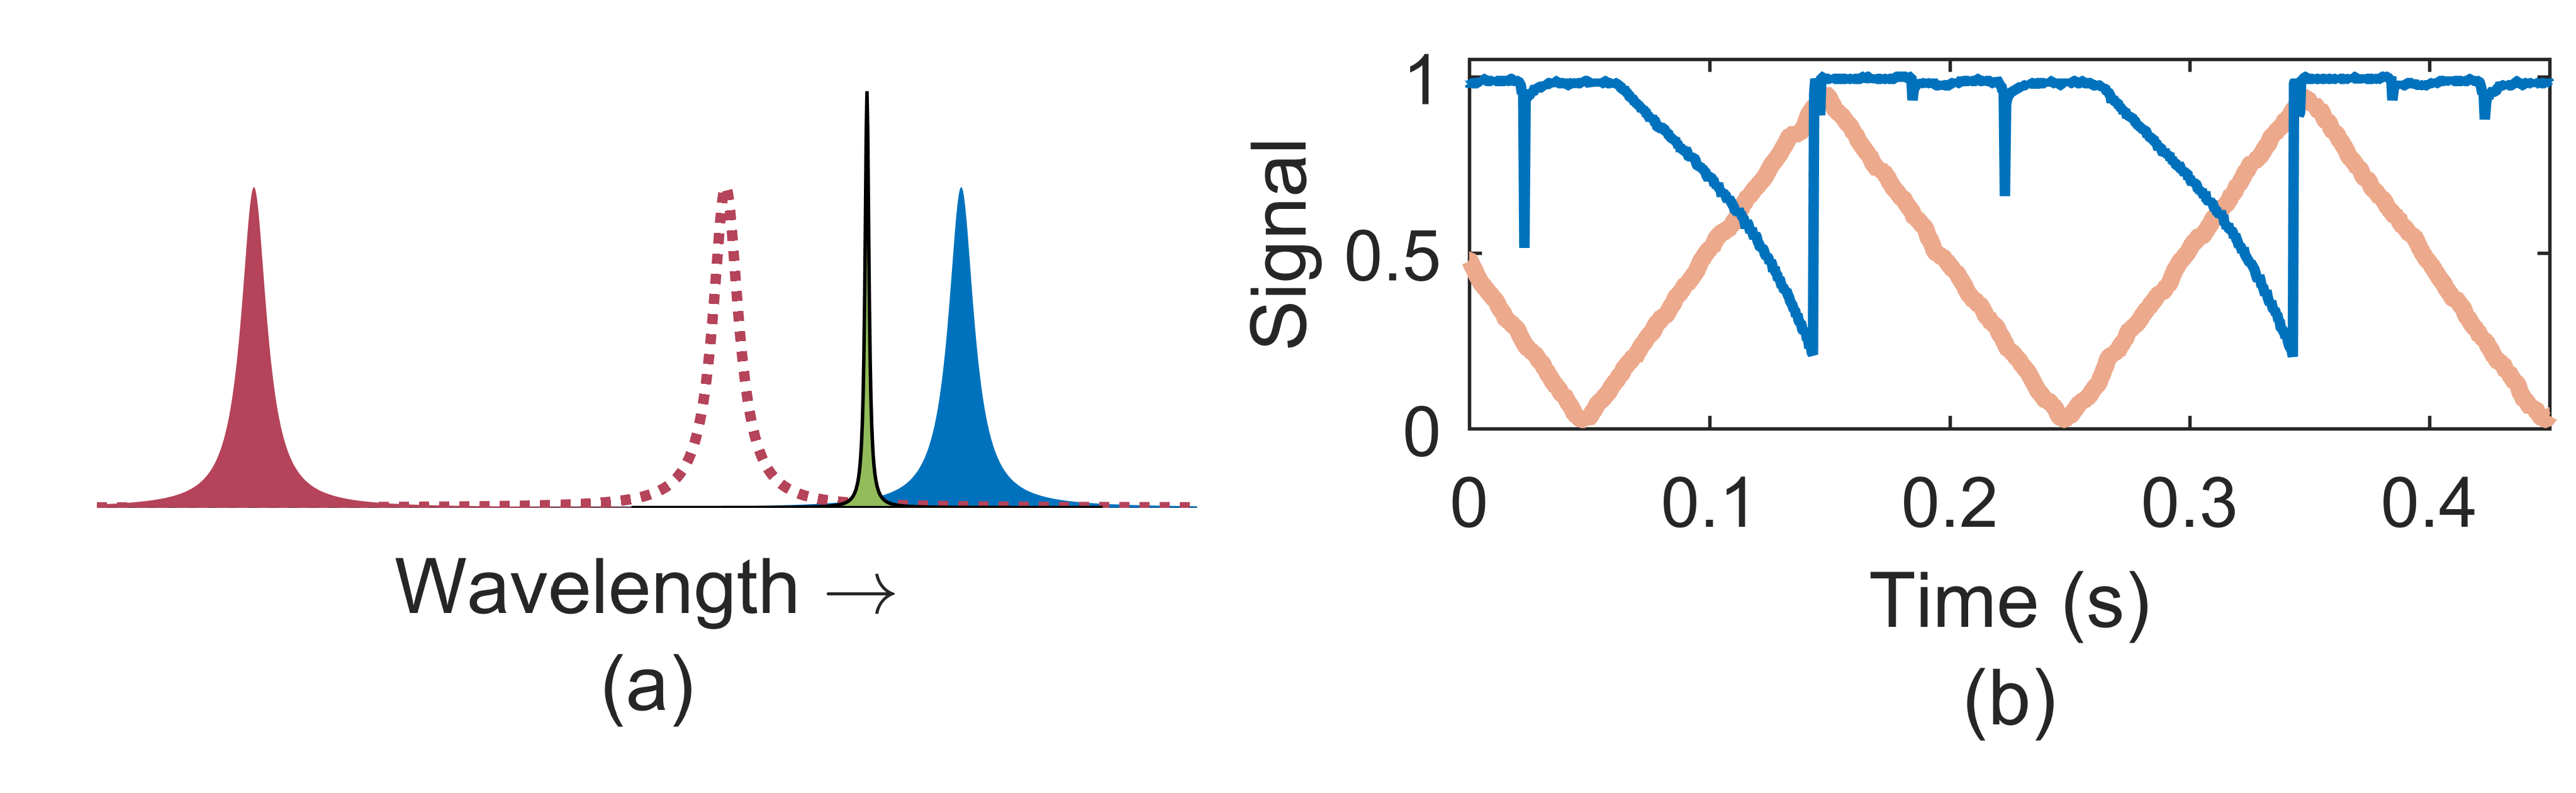
\includegraphics{\FigPath/Figures/Microresonators/MRthermal.png}
%	\end{center}
%	\caption[Thermal bistability in microresonators]{\textbf{Thermal bistability in microresonators.} (a) Depiction of the three steady-state points for the laser detuning. For fixed laser wavelength (green), stable steady-state points exist with relatively small blue detuning and significant coupled power (solid blue), and relatively large red detuning and little coupled power (solid red). An unstable steady-state point also exists with red detuning and significant coupled power (dashed red). Note in this terminology that the color of the detuning (red or blue) refers to the position of the laser relative to the position of the resonance in wavelength space. (b)~Measurement of power transmitted past the microresonator in an experiment using a $\sim$16.5 GHz-FSR microdisk resonator and a tapered fiber. The laser wavelength is adjusted by an intracavity piezo-electric crystal. Here, the control signal shown in orange corresponds to longer laser wavelength. As the laser wavelength is increased, the resonator heats and a sawtooth-shaped resonance is observed. As the resonator wavelength is decreased, the system will `flip' from steady-state point (3) to steady-state point (1), leading to observation of a narrow pseudo-Lorentzian resonance, with the exact shape depending on the thermal and scanning timescales.}
%	
%	\label{fig:MRthermal}
%\end{figure} 

\begin{figure}[htpb]
	\begin{center}
		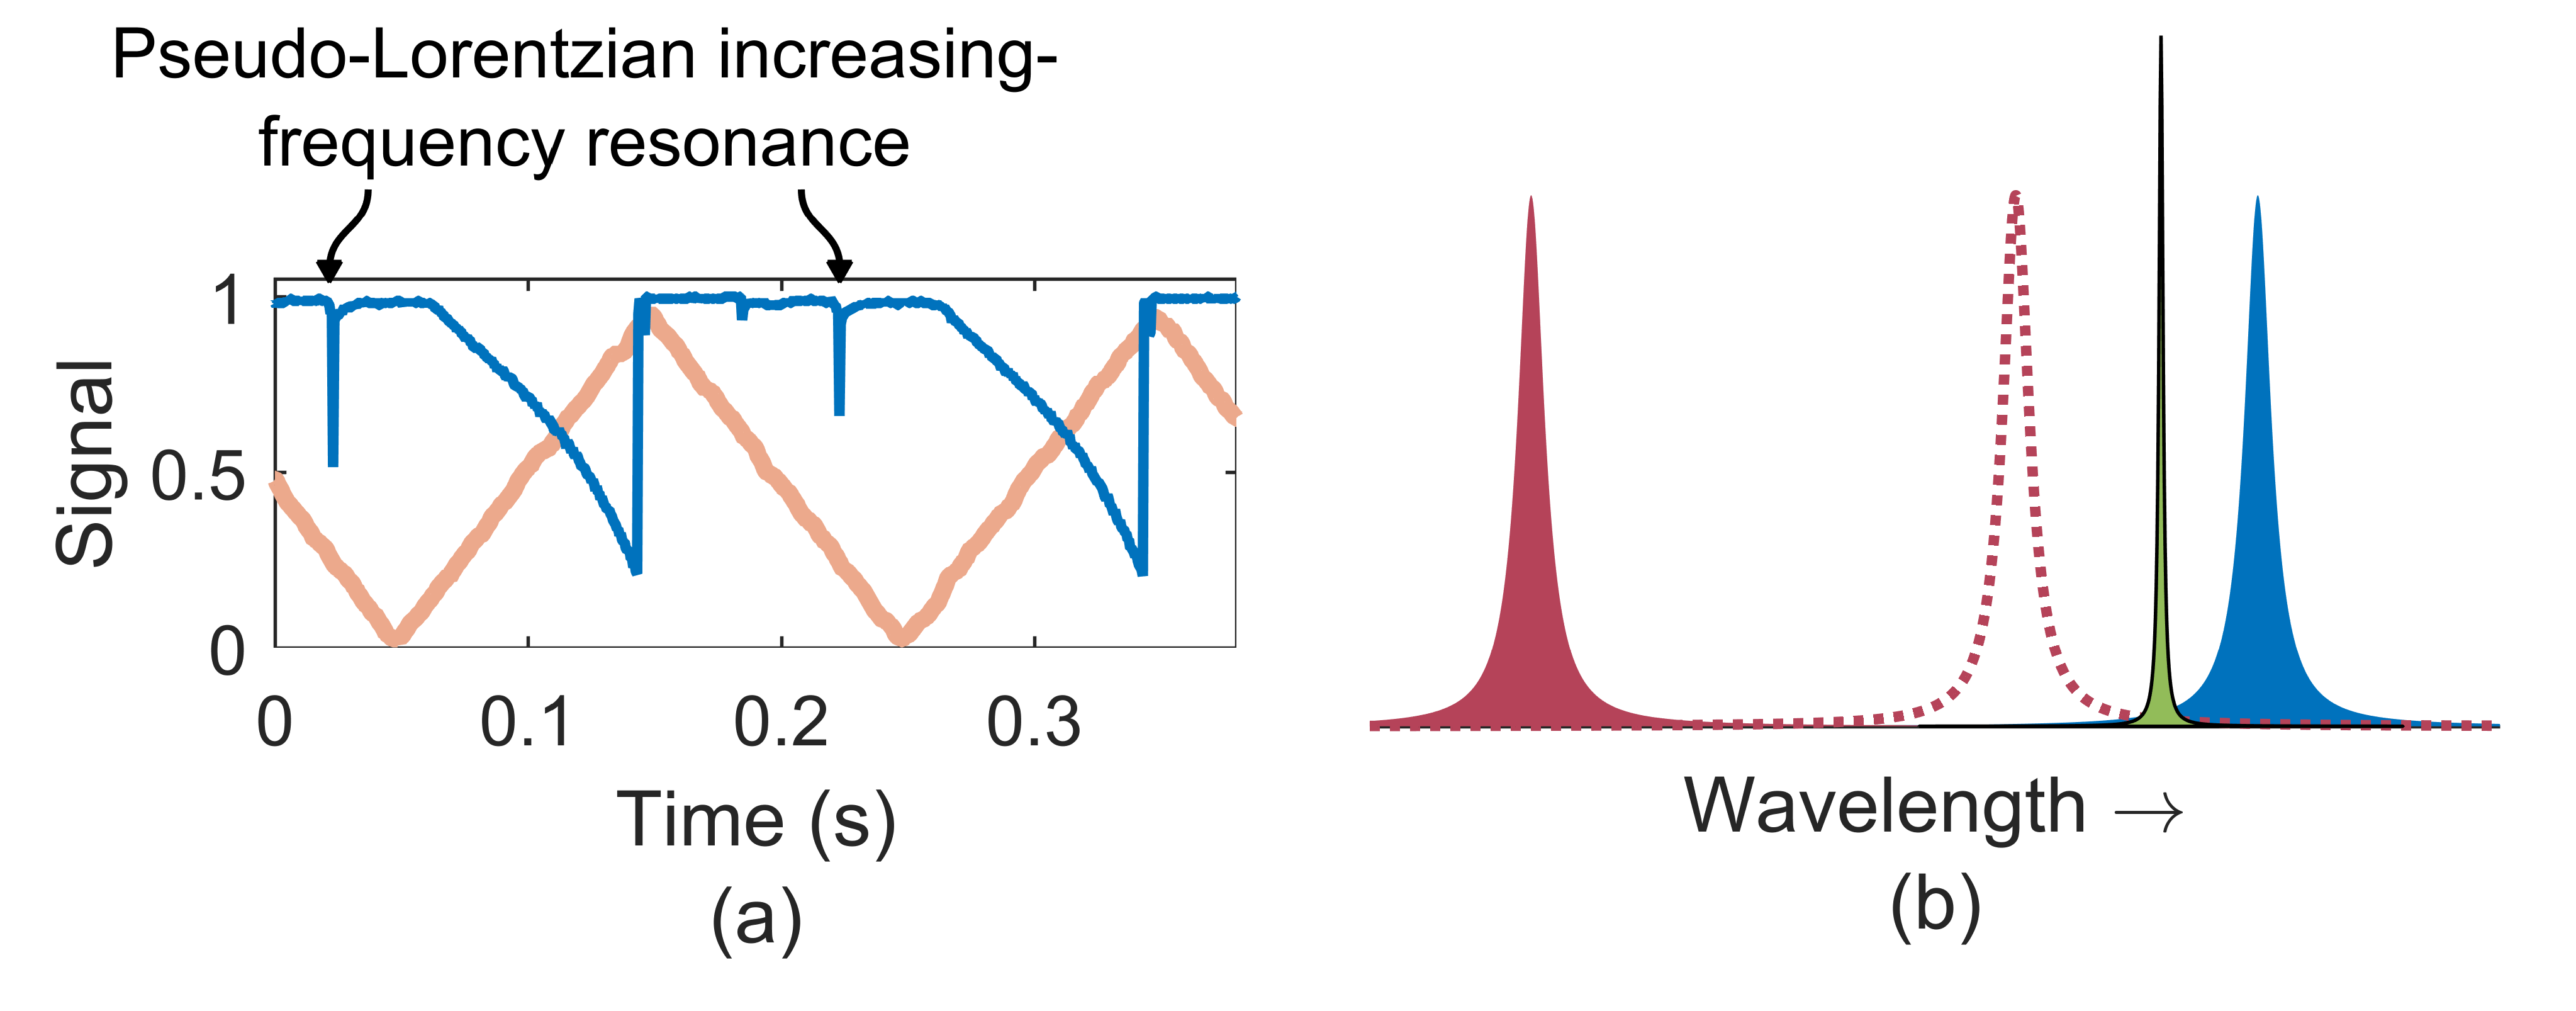
\includegraphics{\FigPath/Figures/Microresonators/MRthermalv4.png}
	\end{center}
	\caption[Thermal bistability in microresonators]{\textbf{Thermal bistability in microresonators.} (a)~Measurement of power transmitted past the microresonator (blue) in an experiment using a $\sim$16.5 GHz-FSR microdisk resonator and a tapered fiber. The wavelength of the pump laser is controlled by a piezo-electric crystal that adjusts the length of the laser cavity. Here, larger control signal (orange) corresponds to longer laser wavelength. As the laser wavelength is increased, the resonator heats and a sawtooth-shaped resonance is observed. Ultimately the resonator reaches a maximum temperature that depends on the pump power, and the laser then becomes red-detuned as the wavelength continues to increase; then the resonator rapidly cools and the resonance is lost. Shortly thereafter, the direction of the scan is reversed. As the resonator wavelength is decreased, the system will `flip' from steady-state point (3) to steady-state point (1), leading to observation of a narrow pseudo-Lorentzian resonance, with the exact shape depending on the thermal and scanning timescales. (b) Depiction of the three steady-state points for the laser detuning. For fixed laser wavelength (green), stable steady-state points exist with relatively small blue detuning and significant coupled power (solid blue), and relatively large red detuning and little coupled power (solid red). An unstable steady-state point also exists with red detuning and significant coupled power (dashed red). Note in this terminology that the color of the detuning (red or blue) refers to the position of the laser relative to the position of the resonance in wavelength space. }
	
	\label{fig:MRthermal}
\end{figure} 








\section{Microring resonator Kerr frequency combs}

The high circulating optical intensities accessible in resonators with long photon lifetimes find immediate application in the use of microresonators for nonlinear optics. The experiments described in this thesis are conducted in silica microresonators. Silica falls into a broader class of materials that exhibit both centro-symmetry, which dictates that the second-order nonlinear susceptibility $\chi^{(2)}$ must vanish, and a significant third-order susceptibility $\chi^{(3)}$. The $n$\textsuperscript{th}-order susceptibility is a term in the Taylor expansion describing the response of the medium's polarization to an external electric field \cite{Boyd2003}: $P=P_0+\epsilon_0 \chi^{(1)} E + \epsilon_0 \chi^{(2)} E^2 + \epsilon_0 \chi^{(3)} E^3+...$. The effect of $\chi^{(3)}$ can be described in a straightforward way as a dependence of the refractive index on the local intensity \cite{Agrawal2007},
\begin{equation}
n=n_0+n_2 I \label{eq:KerrIndex}
\end{equation}
where $n_2=\frac{3\chi^{(3)}}{4n_0^2\epsilon_0 c}$ is called the Kerr index \cite{DelCoso2004,Agrawal2007}. The intensity-dependence of the refractive index resulting from the third-order susceptibility $\chi^{(3)}$ is referred to as the optical Kerr effect and enables the self-phase modulation, cross-phase modulation, and four-wave mixing (FWM) nonlinear processes, the last of which is depicted schematically in Fig. \ref{fig:MRfwm} \cite{Boyd2003}. 

\begin{figure}[htpb]
	\begin{center}
		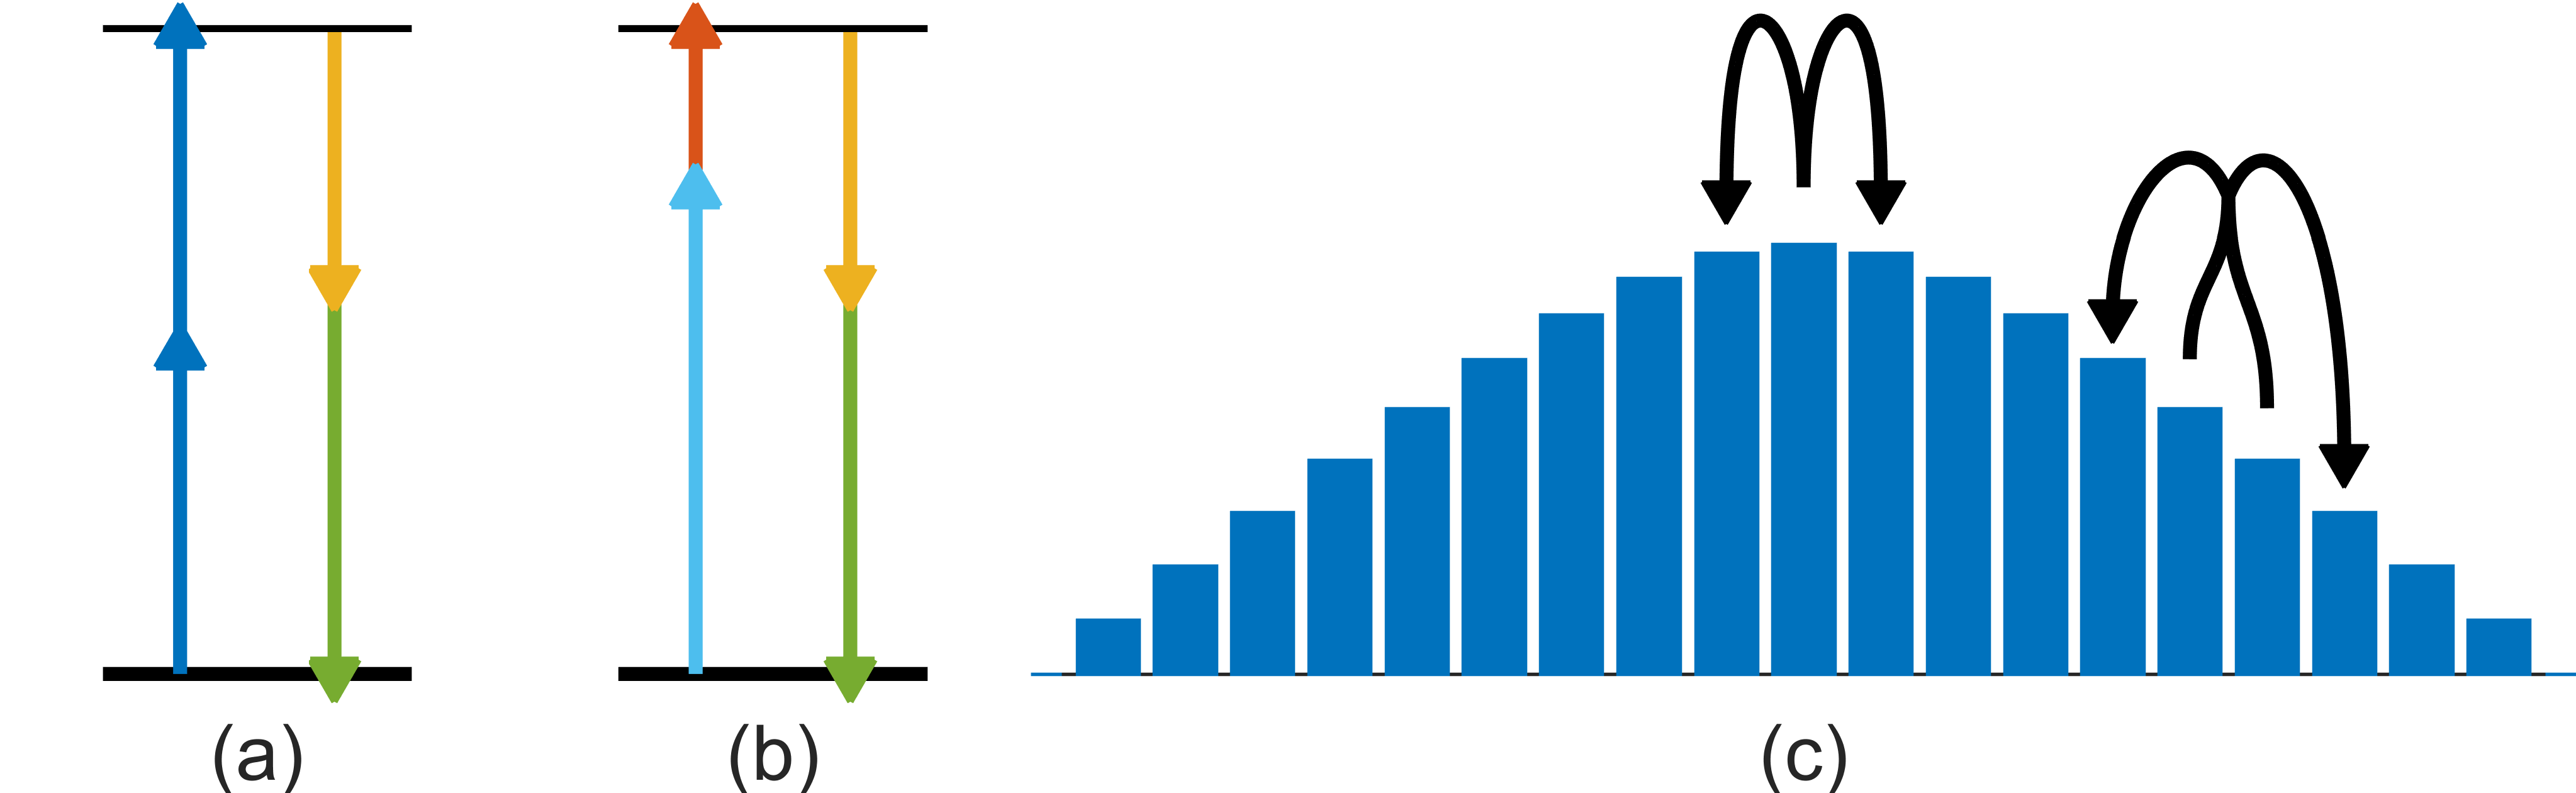
\includegraphics{\FigPath/Figures/Microresonators/MRfwm.png}
	\end{center}
	\caption[An illustration of four-wave mixing and frequency-comb generation.]{\textbf{An illustration of four-wave mixing and frequency-comb generation.} (a)~Degenerate four-wave mixing, in which two fields of the same frequency $\omega_1$ (blue) mix and generate fields at two new frequencies $\omega'$ and $\omega''$ (yellow and green). The schematic indicates the energy-conversation requirements of the process, which can be written as $2\omega_1=\omega'+\omega''$. (b) Non-degenerate four-wave mixing, in which two fields of different frequencies $\omega_2$ and $\omega_3$ (light blue and orange) mix to generate fields at frequencies $\omega'$ and $\omega''$ (yellow and green). Energy conservation is now expressed as $\omega_2+\omega_3=\omega'+\omega''$. (c) Schematic depiction of one degenerate FWM step and one non-degenerate FWM step in a cascaded four-wave mixing process that generates a frequency comb. \footnotesize{Figure after Ref. \cite{Kippenberg2011}.}}
	
	\label{fig:MRfwm}
\end{figure} 


%Measurements indicated that the frequency spacing was uniform to a precision of $7.3 \times 10^{-18}$, thereby establishing that the output of the system was a frequency comb.

In 2007, a remarkable result brought about a new era for frequency comb research. Del'Haye et al. reported \textit{cascaded four-wave mixing} (CFWM, shown in Fig. \ref{fig:MRfwm}c) in anomalously-dispersive ($\beta_{prop,2}=\frac{\partial^2\beta_{prop}(\omega)}{\partial\omega^2}<0$) toroidal silica microcavities on silicon chips, the result of which was a set of many co-circulating optical fields that were uniformly spaced by $f_{rep}$ ranging from 375 GHz to $\sim$750 GHz (depending on the platform) \cite{DelHaye2007}. This result built on previous demonstrations of few-mode parametric oscillation in microresonators \cite{Kippenberg2004, Savchenkov2004,Agha2007}, and showed that the non-uniform distribution of cavity resonance frequencies due to dispersion could be overcome to generate an output with equidistant frequency modes. A second important development occurred in 2012, when Herr et al. reported the generation of frequency combs corresponding in the time domain to single circulating optical `soliton' pulses \cite{Herr2012a,Herr2014}. This observation followed the observation of solitons in formally-equivalent passive fiber-ring resonators in 2010 \cite{Leo2010a}. Due to unique properties that make them particularly well-suited for applications, as discussed in Sec. \ref{sec:LLEsolitons}, the generation and manipulation of soliton combs has become a significant priority in microcomb research. 

\subsection{A model for Kerr-comb nonlinear optics: The Lugiato-Lefever equation}

Kerr-comb generation can be motivated and partially understood through the CFWM picture \cite{Herr2012}, but the phase and amplitude degrees of freedom for each comb line mean that CFWM gives rise to a rich space of comb phenomena---it is now known that Kerr combs can exhibit several fundamentally distinct outputs.  A useful model for understanding this rich space is the Lugiato-Lefever equation (LLE), which was shown to describe microcomb dynamics by Chembo and Menyuk \cite{Chembo2013} through Fourier-transformation of a set of coupled-mode equations describing CFWM and by Coen, Randle, Sylvestre, and Erkintalo \cite{Coen2013a} through time-averaging of a more formally-accurate model for a low-loss resonator (as first performed by Haelterman, Trillo, and Wabnitz \cite{Haelterman1992a}).  The LLE is a nonlinear partial-differential equation that describes evolution of the normalized cavity field envelope $\psi$ over a slow time $\tau=t/2\tau_{ph}$ in a frame parametrized by the ring's azimuthal angle $\theta$ (running from $-\pi$ to $\pi$) co-moving at the group velocity.\footnote{The co-moving azimuthal angle $\theta$ is analogous to the `fast time' variable that appears in, for example, the nonlinear Schrodinger equation for fiber-optic pulse propagation \cite{Agrawal2007}, and it can be transformed explicitly to a fast time $t$ via $t=T_{RT}\times\frac{\theta}{2\pi}$.} The equation formulated by Chembo and Menyuk, as it will be used throughout this thesis, reads:
\begin{equation}
\frac{\partial \psi}{\partial \tau}=-(1+i \alpha) \psi + i|\psi|^2 \psi -i \frac{\beta_2}{2} \frac{\partial^2 \psi}{\partial \theta^2} +F. \label{eq:LLE}
\end{equation}

This equation describes $\psi$ over the domain $-\pi\leq\theta\leq+\pi$ with periodic boundary conditions $\psi(-\pi,\tau)=\psi(\pi,\tau)$. Here $F$ is the field strength of the pump laser, with $F$ and $\psi$ both normalized so that they  take the value 1 at the absolute threshold for parametric oscillation: $F=\sqrt{\frac{8 g_0\Delta\omega_{ext}}{\Delta\omega_{tot}^3}\frac{P_{in}}{\hbar \wpl}}$, $|\psi|^2=\frac{2g_0T_{RT}}{\hbar\wpl\Delta\omega_{tot}}P_{circ}(\theta,\tau)$, so that $|\psi(\theta,\tau)|^2$ is the instantaneous normalized power at the co-moving azimuthal angle $\theta$. Here $g_0=n_2 c \hbar \wpl^2/n_g^2 V_0$ is a parameter describing the four-wave mixing gain, $\Delta\omega_{ext}$ is the rate of coupling at the input/output port, $\Delta\omega_{tot}=1/\tau_{ph}$ is the FWHM resonance linewidth, $P_{in}$ is the pump-laser power, $P_{circ}(\theta,\tau)$ is the local circulating power in the cavity, $\hbar$ is Planck's constant, and $\wpl$ is the pump-laser frequency. The parameters $n_2$, $n_g$, and $V_0$ describe the nonlinear (Kerr) index (see Eqn. \ref{eq:KerrIndex}), the group index of the mode, and the effective nonlinear mode volume at the pump frequency; $L$ is the physical round-trip length of the ring cavity. 

The parameters $\alpha$ and $\beta_2$ describe the frequency detuning of the pump laser and second-order dispersion of the resonator mode family into which the pump laser is coupled, both normalized to half the cavity linewidth: 
\begin{align}
\alpha&=-\frac{2(\wpl-\omega_0)}{\Delta\omega_{tot}},\\
\beta_2&=-\frac{2 D_2}{\Delta\omega_{tot}};
\end{align} here $D_2=\left.\frac{\partial^2\omega_\mu}{\partial \mu^2}\right|_{\mu=0}$ is the second-order modal dispersion parameter, where $\mu$ is the pump-referenced mode number of Eq. \ref{eq:combfreqsnew}. The parameters $D_1=\left.\frac{\partial\omega_\mu}{\partial\mu}\right|_{\mu=0}=2\pi f_{FSR}$ and $D_2$ are related to the derivatives of the propagation constant $\beta_{prop}=n_{eff}(\omega)\omega/c$ via $D_1=2\pi/L\beta_1$ and $D_2=-D_1^2\frac{\beta_{prop,2}}{\beta_{prop,1}}$, where $\beta_{prop,n}=\partial^n\beta_{prop}/\partial\omega^n$. The subscript $prop$ is used here to distinguish the propagation constant from the LLE dispersion coefficients $\beta_n=-2D_n/\Delta\omega_{tot}$, as unfortunately the use of the symbol $\beta$ for both of these quantities is standard. Expressions for higher-order modal dispersion parameters $D_n$ in terms of the expansion of the propagation constant can be obtained by evaluating the equation $D_{n>1}=(D_1\frac{\partial}{\partial \omega})^{n-1} D_1$, and may be incorporated into the LLE up to desired order $N$ through the replacement:
\begin{equation}
-i\frac{\beta_2}{2}\frac{\partial^2\psi}{\partial\theta^2}\rightarrow +\sum_{n=1}^N i^{n+1} \frac{\beta_n}{n!}\frac{\partial^n\psi}{\partial\theta^n}.
\end{equation}
This thesis describes frequency-comb generation in anomalously-dispersive resonators, and so $\beta_2<0$ throughout.

The formulation of the LLE in terms of dimensionless normalized parameters helps to elucidate the fundamental properties of the system and facilitates comparison of results obtained in platforms with widely different experimental conditions. The LLE relates the time-evolution of the intracavity field (normalized to its threshold value for cascaded four-wave mixing) to the power of the pump laser (normalized to its value at the threshold for cascaded four-wave mixing), the pump-laser detuning (normalized to half the cavity linewidth), and the cavity second-order disperison quantified by the change in the FSR per mode (normalized to half the cavity linewidth). One example of the utility of this formulation is that it makes apparent the significance of the cavity linewidth in determining the output comb, and underscores the fact that optimization of the dispersion, for example, without paying heed to the effect of this optimization on the cavity linewidth, may not yield the desired results. This adds an additional layer of complexity to dispersion engineering relative to straight waveguides.

The LLE is, of course, a simplified description of the dynamics occurring in the microresonator. It abstracts the nonlinear dynamics and generally successfully describes the various outputs that can be generated in a microresonator frequency comb experiment. The LLE is a good description of these nonlinear dynamics when the resonator photon lifetime, mode overlap, and nonlinear index $n_2$ are roughly constant over the bandwidth of the generated comb, and when the dominant contribution to nonlinear dynamics is simply the self-phase modulation term $i|\psi|^2\psi$ arising from the Kerr nonlinearity. The LLE neglects the polarization of the electric field ($\psi$ is a scalar), as well as thermal effects and the Raman scattering and self-steepening nonlinearities, although in principle each of these can be included \cite{Hansson2018,Herr2014,Chembo2015,Agrawal2007}. It is also worth emphasizing that the LLE can be derived from a more formally-accurate Ikeda map (as explained by Coen et al. \cite{Coen2013a}), in which the effect of localized input- and output-coupling is included in the model. This derivation is accomplished by `delocalizing' the pump field and the output-coupling over the round trip, including only their averaged effects. This is an approximation that is valid in the limit of high finesse due to the fact that the cavity field cannot change on the timescale of a single round trip, but as a result the LLE necessarily neglects all dynamics that might have some periodicity at the round-trip time; the fundamental timescale of LLE dynamics is the photon lifetime. 




%The LLE provides a useful framework for the prediction of comb properties and the exploration of avenues for new research, but also has proven to be an important tool in the interpretation of Kerr-comb experimental results. A primary reason for this is the difficulty of directly characterizing the time-domain output of a microresonator---typically, available tools enable measurement of time-averaged optical spectra and measurement of the comb's output power within the bandwidth of the photodetectors (generally $\lesssim$ 50 GHz) and amplifiers used for the measurement. Since neither records phase information and the latter lacks response on the timescale of, e.g., temporal pulses with duration less than a microresonator's round-trip time, these measurements are insufficient to determine the time-domain output of the microresonator. By providing a mathematical formalism that restricts the possible behaviors of the intracavity field $\psi$, the LLE enables inference of the temporal intensity profile $|\psi(\theta,\tau)|^2$ from the spectrum $|\psi_\mu(\tau)|^2$, which is readily measured in experiment.  \todo{How does FROG fit into this discussion?}

\section{Description of Kerr-comb outputs using the Lugiato-Lefever equation}

The LLE provides a useful framework for the prediction and interpretation of experimental results. Basically, it predicts the existence of two fundamentally distinct types of Kerr-combs: extended temporal patterns and localized soliton pulses. These predictions are born out by experiments, the interpretation of which is facilitated by insight gained from the LLE. In the remainder of this chapter I briefly present some analytical results that can be obtained from the LLE about the behavior of the continuous-wave (CW) field that exists in the resonator in the absence of Kerr-comb formation, and then discuss these two types of comb outputs. This discussion provides context for the results presented in the next two chapters. Fig. \ref{fig:MRLLEspace} summarizes the results that will be presented in the remainder of this chapter, and in particular shows the values of the parameters $\alpha$ and $F^2$ at which solitons and extended patterns can be obtained.



\begin{figure}[htpb]
	\begin{center}
		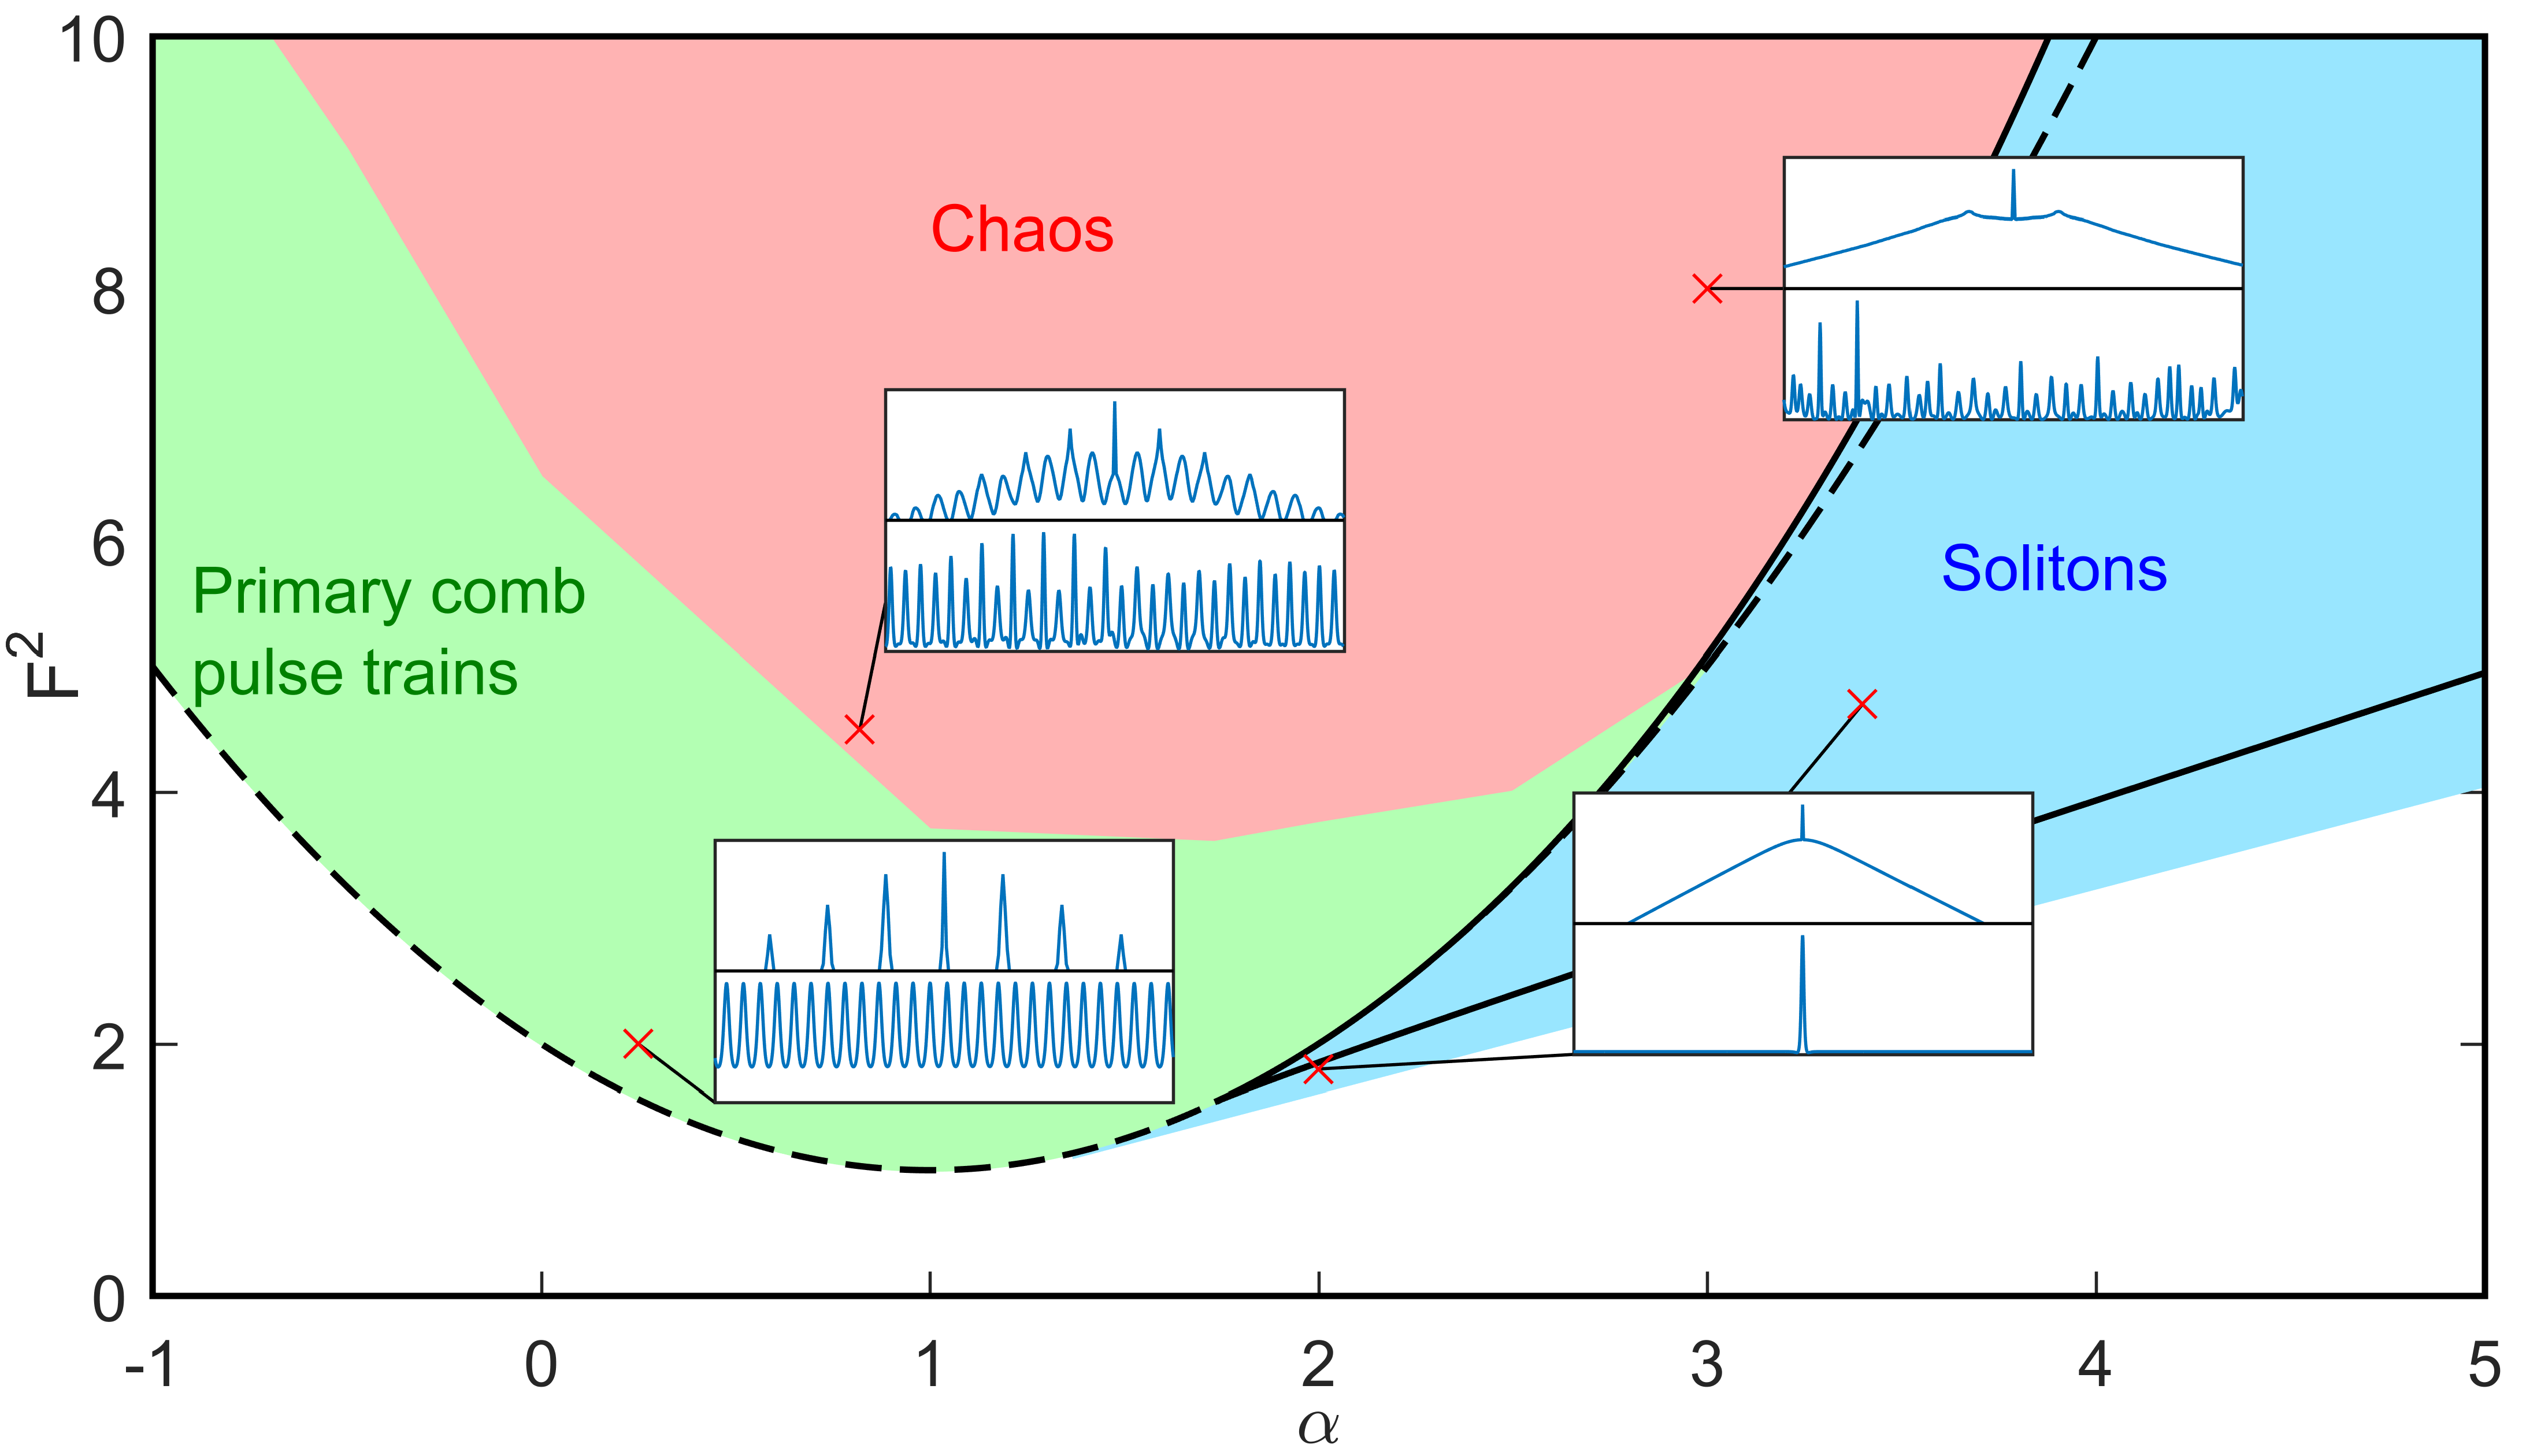
\includegraphics{\FigPath/Figures/Microresonators/MRLLEspace.png}
	\end{center}
	\caption[Solution space for the Lugiato-Lefever equation]{\textbf{Solution space for the Lugiato-Lefever equation.} Depiction of the various behaviors exhibited by $\psi$ as a function of its position in the $\alpha-F^2$ plane; this predicts the type of Kerr-comb output as a function of the pump-laser detuning and power, the parameters that are most readily adjusted in experiment. Curves plotted in black are obtained through analytical investigation of the LLE; these include the threshold curve for parametric oscillation (dashed black, Eq. \ref{eq:F2thresh}) and the lines obtained via $\rho(\alpha,F^2)=\rho_\pm(\alpha)$ (solid black, Eq. \ref{eq:rhopm}), which define the region where the LLE exhibits multiple flat solutions (i.e. solutions such that $\partial \psi/\partial \theta=0$, Eq. \ref{eq:LLEstat}). Extended patterns arise above the threshold curve through modulation instability. Solitons exist outside of the threshold curve at higher red detuning, up to an approximate maximum $\alpha_{max}=\pi^2 F^2/8$. The lines bounding the existence of chaos are not known precisely, and in fact chaos can be observed in simulation outside of the threshold curve at values $\alpha>\alpha_{thresh,+}$ (Eq. \ref{eq:alphathresh}). Insets show representative simulation results for the various types of comb outputs in the frequency (top) and time (bottom) domains. \footnotesize{Fig. after Ref. \cite{Godey2014}}.
	 }
	
	\label{fig:MRLLEspace}
\end{figure} 



%
%In the following subsections I introduce two fundamentally-distinct types of Kerr-combs. This provides important context for the results presented in the next two chapters. 

\subsection{Analytical investigation of the resonator's CW response}\label{sec:MRanalyticalcurves}
Some insight into comb dynamics can be obtained via analytical investigations of the LLE, Eq. \ref{eq:LLE}. This section largely follows the analysis of Ref. \cite{Godey2014}, with similar analysis having been performed elsewhere, for example in Refs. \cite{Coen2013a} and \cite{Barashenkov1996}. When the derivative term $\partial^2\psi/\partial\theta^2$ in the LLE is non-zero, $\psi$ is necessarily broadband, and a Kerr comb has been formed. There are no known exact analytical solutions to the LLE to describe Kerr-comb outputs, which must instead be numerically simulated (see App. \ref{app:numericalsims}). However, flat solutions $\psi_{CW}$ to the LLE  may be calculated by setting all derivatives to zero---when these solutions can be realized physically (discussed below), they describe a CW field in the resonator. Upon setting the derivatives in the LLE to zero, one finds:
\begin{equation}
F=(1+i\alpha)\psi_{CW}-i|\psi_{CW}|^2\psi_{CW}. \label{eq:LLEstat}
\end{equation}
The circulating intensity $\rho=|\psi_{CW}|^2$ is obtained by taking the modulus-square of Eq. \ref{eq:LLEstat} to obtain:
\begin{align}
F^2&=\left(1+(\alpha-\rho)^2\right)\rho\label{eq:LLEstat2},\\
&=\rho^3-2\alpha\rho^2+(\alpha^2+1)\rho,
\end{align} 
whereupon this equation can be numerically solved for $\rho$. As a third-order polynomial in $\rho$ this equation has three solutions, one or three of which may be real; the complex solutions are unphysical. The function $F^2(\alpha,\rho)$ defined by this equation uniquely determines $F^2$ given $\alpha$ and $\rho$. We now consider plotting a graph of $F^2(\alpha,\rho)$ with $\alpha$ held constant; examples are given in Fig. \ref{fig:MRcurves}. By noting that $F^2(\alpha,\rho=0)=0$ and $\left.\partial F^2/\partial \rho\right|_{\rho=0}>0$, we can conclude that a graph of $F^2(\alpha,\rho)$ will cross the same value $F^2$ three times if $F^2$ is between the extremal values $F^2_\pm(\alpha)$ at which $\partial F^2/\partial\rho=0$. This means that three real solutions $\rho_1$, $\rho_2$, and $\rho_3$ for the inverted function $\rho(\alpha,F^2)$ exist for each value of $F^2$ between $F^2_-(\alpha)$ and $F^2_+(\alpha)$. The values $F^2_\pm(\alpha)$ bounding  this region of degeneracy in $\rho$ are found by inserting the values $\rho_\pm$ at which $\partial F^2/\partial\rho=0$ into Eq. \ref{eq:LLEstat2}. That is, $F^2_\pm(\alpha)=F^2(\alpha,\rho_\mp)$, where:
\begin{equation}
\rho_\pm=\frac{2\alpha\pm\sqrt{\alpha^2-3}}{3}.\label{eq:rhopm}
\end{equation}
For pump powers outside of the interval $[F^2_-(\alpha),F^2_+(\alpha)]$, which varies with $\alpha$, there is only one real solution $\rho$; within this interval there are three. This is illustrated in Fig. \ref{fig:MRcurves}. The smallest value of $F^2$ at which the stationary curve $\rho$ becomes multivalued is found to be $F^2=8\sqrt{3}/9$ by solving for $\rho_-=\rho_+$ and inserting the corresponding values into Eq. \ref{eq:LLEstat2}.

\begin{figure}[htpb]
	\begin{center}
		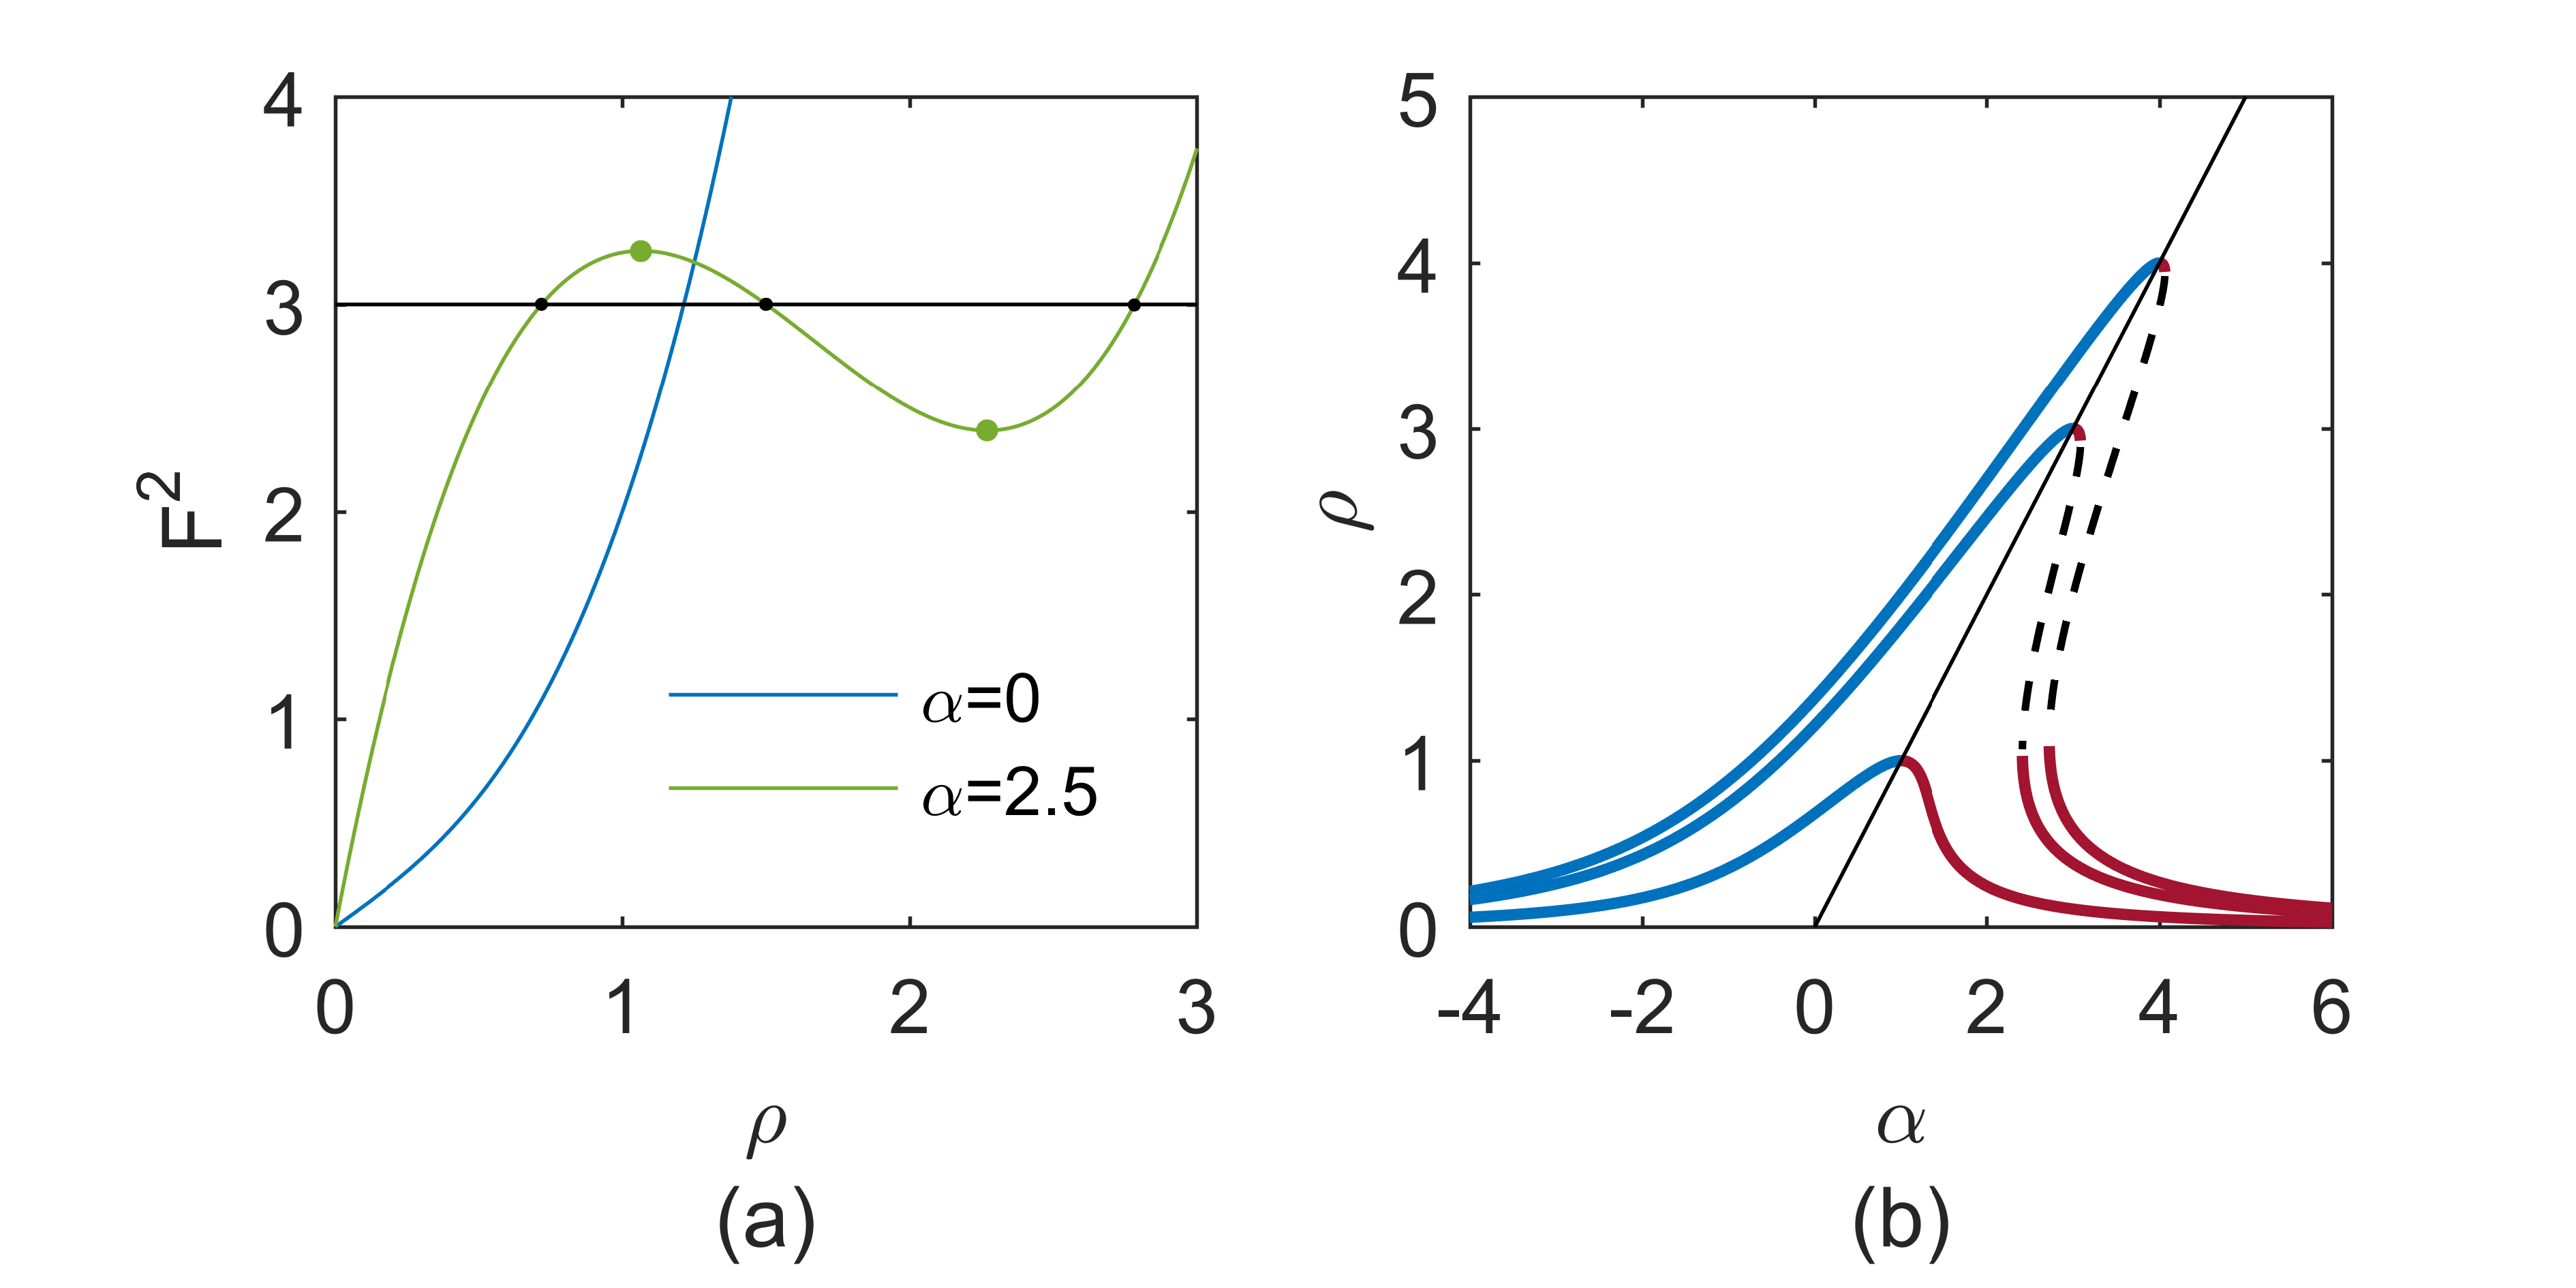
\includegraphics{\FigPath/Figures/Microresonators/MRcurves.png}
	\end{center}
	\caption[Investigation of the circulating CW power in a Kerr resonator]{\textbf{Investigation of the circulating CW power in a Kerr resonator.} (a) Plots of $F^2$ as a function of $\rho$ for $\alpha=0$ (blue) and $\alpha=2.5$ (green), according to Eq. \ref{eq:LLEstat2}. When real values of $\rho$ exist that extremize $F^2$ according to this equation, multiple real solutions for the circulating power $\rho$ exist between these extremal values of $F^2$. For $\alpha=2.5$ we indicate the extremal values of $F^2$ as green dots. For an example value $F^2=3$, the corresponding allowed values $\rho_1$, $\rho_2$, and $\rho_3$ are the intersections of the green curve and the black line (black dots); such a line would have three intersections with the green curve for any value of $F^2$ between $F^2_\alpha(\rho_-)$ and $F^2_\alpha(\rho_+)$. (b) Kerr-tilted resonances curves $\rho(\alpha)$ for $F^2=$1 (smallest), $F^2=$3, and $F^2=$4 (largest). The line $\rho=\alpha=F^2$ (solid black) marks the highest circulating power for a given input power $F^2$ and separates the effectively blue-detuned and effectively red-detuned branches. When $F^2>8\sqrt{3}/9$ (obtained by solving for $\rho_+=\rho_-$, Eq. \ref{eq:rhopm}), the resonance becomes tilted steeply enough that an unstable middle branch (dashed black) exists. }
	
	\label{fig:MRcurves}
\end{figure} 

Physically, the coexistence of multiple flat solutions $\rho$ at a given point $(\alpha,F^2)$ corresponds to a `tilting' of the Lorentzian transmission profile of the cavity and leads to bistability, even before taking into account thermal effects. This is illustrated in Fig. \ref{fig:MRcurves}. For flat solutions $\rho$, an effective Kerr-shifted detuning can be defined as $\alpha_{eff}=\alpha-\rho$. The effective detuning simply incorporates the Kerr nonlinearity into the round-trip phase shift that describes the constructive or destructive interference of the circulating field with the pump at the coupling port. By noting that $\alpha=F^2=\rho$ solves Eq. \ref{eq:LLEstat2}, we can conclude that the position of the effective Kerr-shifted resonance is on the line $\alpha=F^2$, where $\alpha_{eff}=0$. 

%For fixed $F^2$, an effectively red-detuned branch of the tilted resonance exists above the value of $\alpha$ where $\rho$ becomes multivalued. This value of $\alpha$ can be determined by inserting $\rho_-$ (Eq. {\ref{eq:rhopm}) into Eq. \ref{eq:LLEstat2} and solving for $\alpha$. 
	
%	The discussion of thermal effects in Sec. \ref{sec:thermaleffects} then applies to the effective detuning $\alpha_{eff}$; that is, operating with significant coupled power at \textit{effective} red detuning is thermally unstable, while thermal locking occurs with significant coupled power at effective blue detuning. 
	
%	Generally speaking, extended patterns exist on the upper branch of this curve, highlighted in blue, and solitons exist on the lower branch, highlighted in red. 

Once the circulating intensity $\rho$ is known, the corresponding flat solution $\psi_{CW}$ can be determined from Eq. \ref{eq:LLEstat} by inserting the known value of $\rho$ and solving for $\psi_{CW}$, with the result:
\begin{equation}
\psi_{CW}=\frac{F}{1+i(\alpha-\rho)}.\label{eq:LLEflatsoln}
\end{equation}
This expression reveals that the flat solution acquires a phase $\phi_s=\tan^{-1}(\rho-\alpha)$ relative to the pump.


%By introducing a perturbation $\delta\psi$ to the flat solution $\psi_s$ and solving for the time evolution of the perturbation, the stability of the flat solution can be investigated---a flat solution $\psi_s$ to the LLE only corresponds to a physically-realizable CW resonator background if it is stable to perturbations. We don't reproduce this analysis in detail here, but state the result:

If the flat solution(s) at a point $(\alpha,F^2)$ is (are) unstable, a Kerr comb will form spontaneously. Stability analysis of the flat solutions can be performed, and for the case of second-order dispersion alone the results are \cite{Godey2014}:
\begin{itemize}
	\item In the region of multi-stability, if the flat solutions are ordered with increasing magnitude as $\rho_1$, $\rho_2$, and $\rho_3$, the middle solution $\rho_2$ is always unstable. 
	\item When $\alpha<2$, a flat solution $\rho$ that is not the middle solution is stable if $\rho<1$; otherwise it is unstable. When the flat solution is unstable, the mode that experiences the greatest instability has mode number given by:
	\begin{equation}
\mu_{max}=\sqrt{\frac{2}{\beta_2}(\alpha-2\rho)}  \label{eq:mumax}
	\end{equation} 
\end{itemize}

Therefore, the pump-laser threshold curve for Kerr-comb generation can be determined in the region $\alpha<2$ of the $\alpha-F^2$ plane by setting $\rho=1$ in Eq. \ref{eq:LLEstat}: 
\begin{equation}
F^2_{thresh}=1+(\alpha-1)^2, \label{eq:F2thresh}
\end{equation}
\begin{equation}
\alpha_{thresh,\pm}=1\pm\sqrt{F^2-1}. \label{eq:alphathresh}
\end{equation}
These equations explicitly describe the point at which comb is generated in an experiment in which the pump power or detuning is varied while the other is held fixed. 



\subsection{Kerr comb outputs: extended modulation-instability patterns}

Extended temporal patterns arise spontaneously as a result of the instability of the flat solution to the LLE when the pump laser is tuned above the threshold curve. Two types of extended patterns are shown in Fig. \ref{fig:MRextendedpatterns}. These patterns can be stationary, in which case they are typically referred to as `Turing patterns' or `primary comb,' or can evolve in time, in which case they are typically referred to as `noisy comb' or `spatiotemporal chaos.' In general, the former occurs for lower values of the detuning $\alpha$ and smaller pump strengths $F^2$; although some studies of the transition from Turing patterns to chaos have been conducted (e.g. Ref. \cite{Coillet2014}), a well-defined boundary between the two has not been established, and may not exist. 

In the spatial domain parametrized by $\theta$, a Turing pattern consists of a pulse train with (typically) $n\gg1$ pulses in the domain $-\pi\leq\theta\leq\pi$---the pulse train's repetition rate is a multiple of the cavity FSR: $f_{rep}=n\times f_{FSR}$. Corresponding to the $n$-fold decreased period (relative to the round-trip time) of an $n$-pulse Turing pattern's modulated waveform in the time domain, the optical spectrum of a Turing pattern consists of modes spaced by $n$ resonator FSR---it is this widely-spaced spectrum that is referred to as `primary comb.'  Analytical approximations for Turing patterns are possible near threshold \cite{Lugiato1987,Lugiato1987a} and in the small damping limit \cite{Renninger2016}. The stability analysis results from the last section can be used to predict the spacing $n$ of a primary comb (equivalently the number of Turing-pattern pulses) generated in a decreasing-frequency scan across the resonance with fixed normalized pump power $F^2$:
\begin{equation}
n=\mu_{max,thresh}=\sqrt{\Delta\omega_0(1+\sqrt{F^2-1})/D_2},
\end{equation}
which is obtained by inserting $\alpha_{thresh,-}$ from Eq. \ref{eq:alphathresh} and $\rho=1$ into the expression for $\mu_{max}$ in Eq. \ref{eq:mumax} above and moving to the dimensionful dispersion parameter $D_2$. Fig. \ref{fig:MRextendedpatterns}a shows measured and simulated primary comb spectra and Fig. \ref{fig:MRextendedpatterns}b shows the corresponding simulated time-domain waveform.

Spatiotemporal chaos can be understood as a Turing pattern whose pulses oscillate in height, with adjacent pulses oscillating out of phase. From such an oscillating Turing pattern, if $\alpha$ and/or $F^2$ is increased, one moves deeper into the chaotic regime and pulses begin to exhibit lateral motion and collisions; the number of pulses present in the cavity is no longer constant in time. Depending on the severity of the chaos (greater for larger $\alpha$ and $F^2$), a chaotic comb may correspond to a primary-comb-type spectrum with each primary-comb mode exhibiting sidebands at the resonator FSR, so-called `subcombs,' or it may correspond to a spectrum with light in each cavity mode. Fig. \ref{fig:MRextendedpatterns}c shows measured and simulated time-averaged spectra of chaotic combs and Fig. \ref{fig:MRextendedpatterns}d shows a corresponding simulated time-domain waveform.

\begin{figure}[htpb]
	\begin{center}
		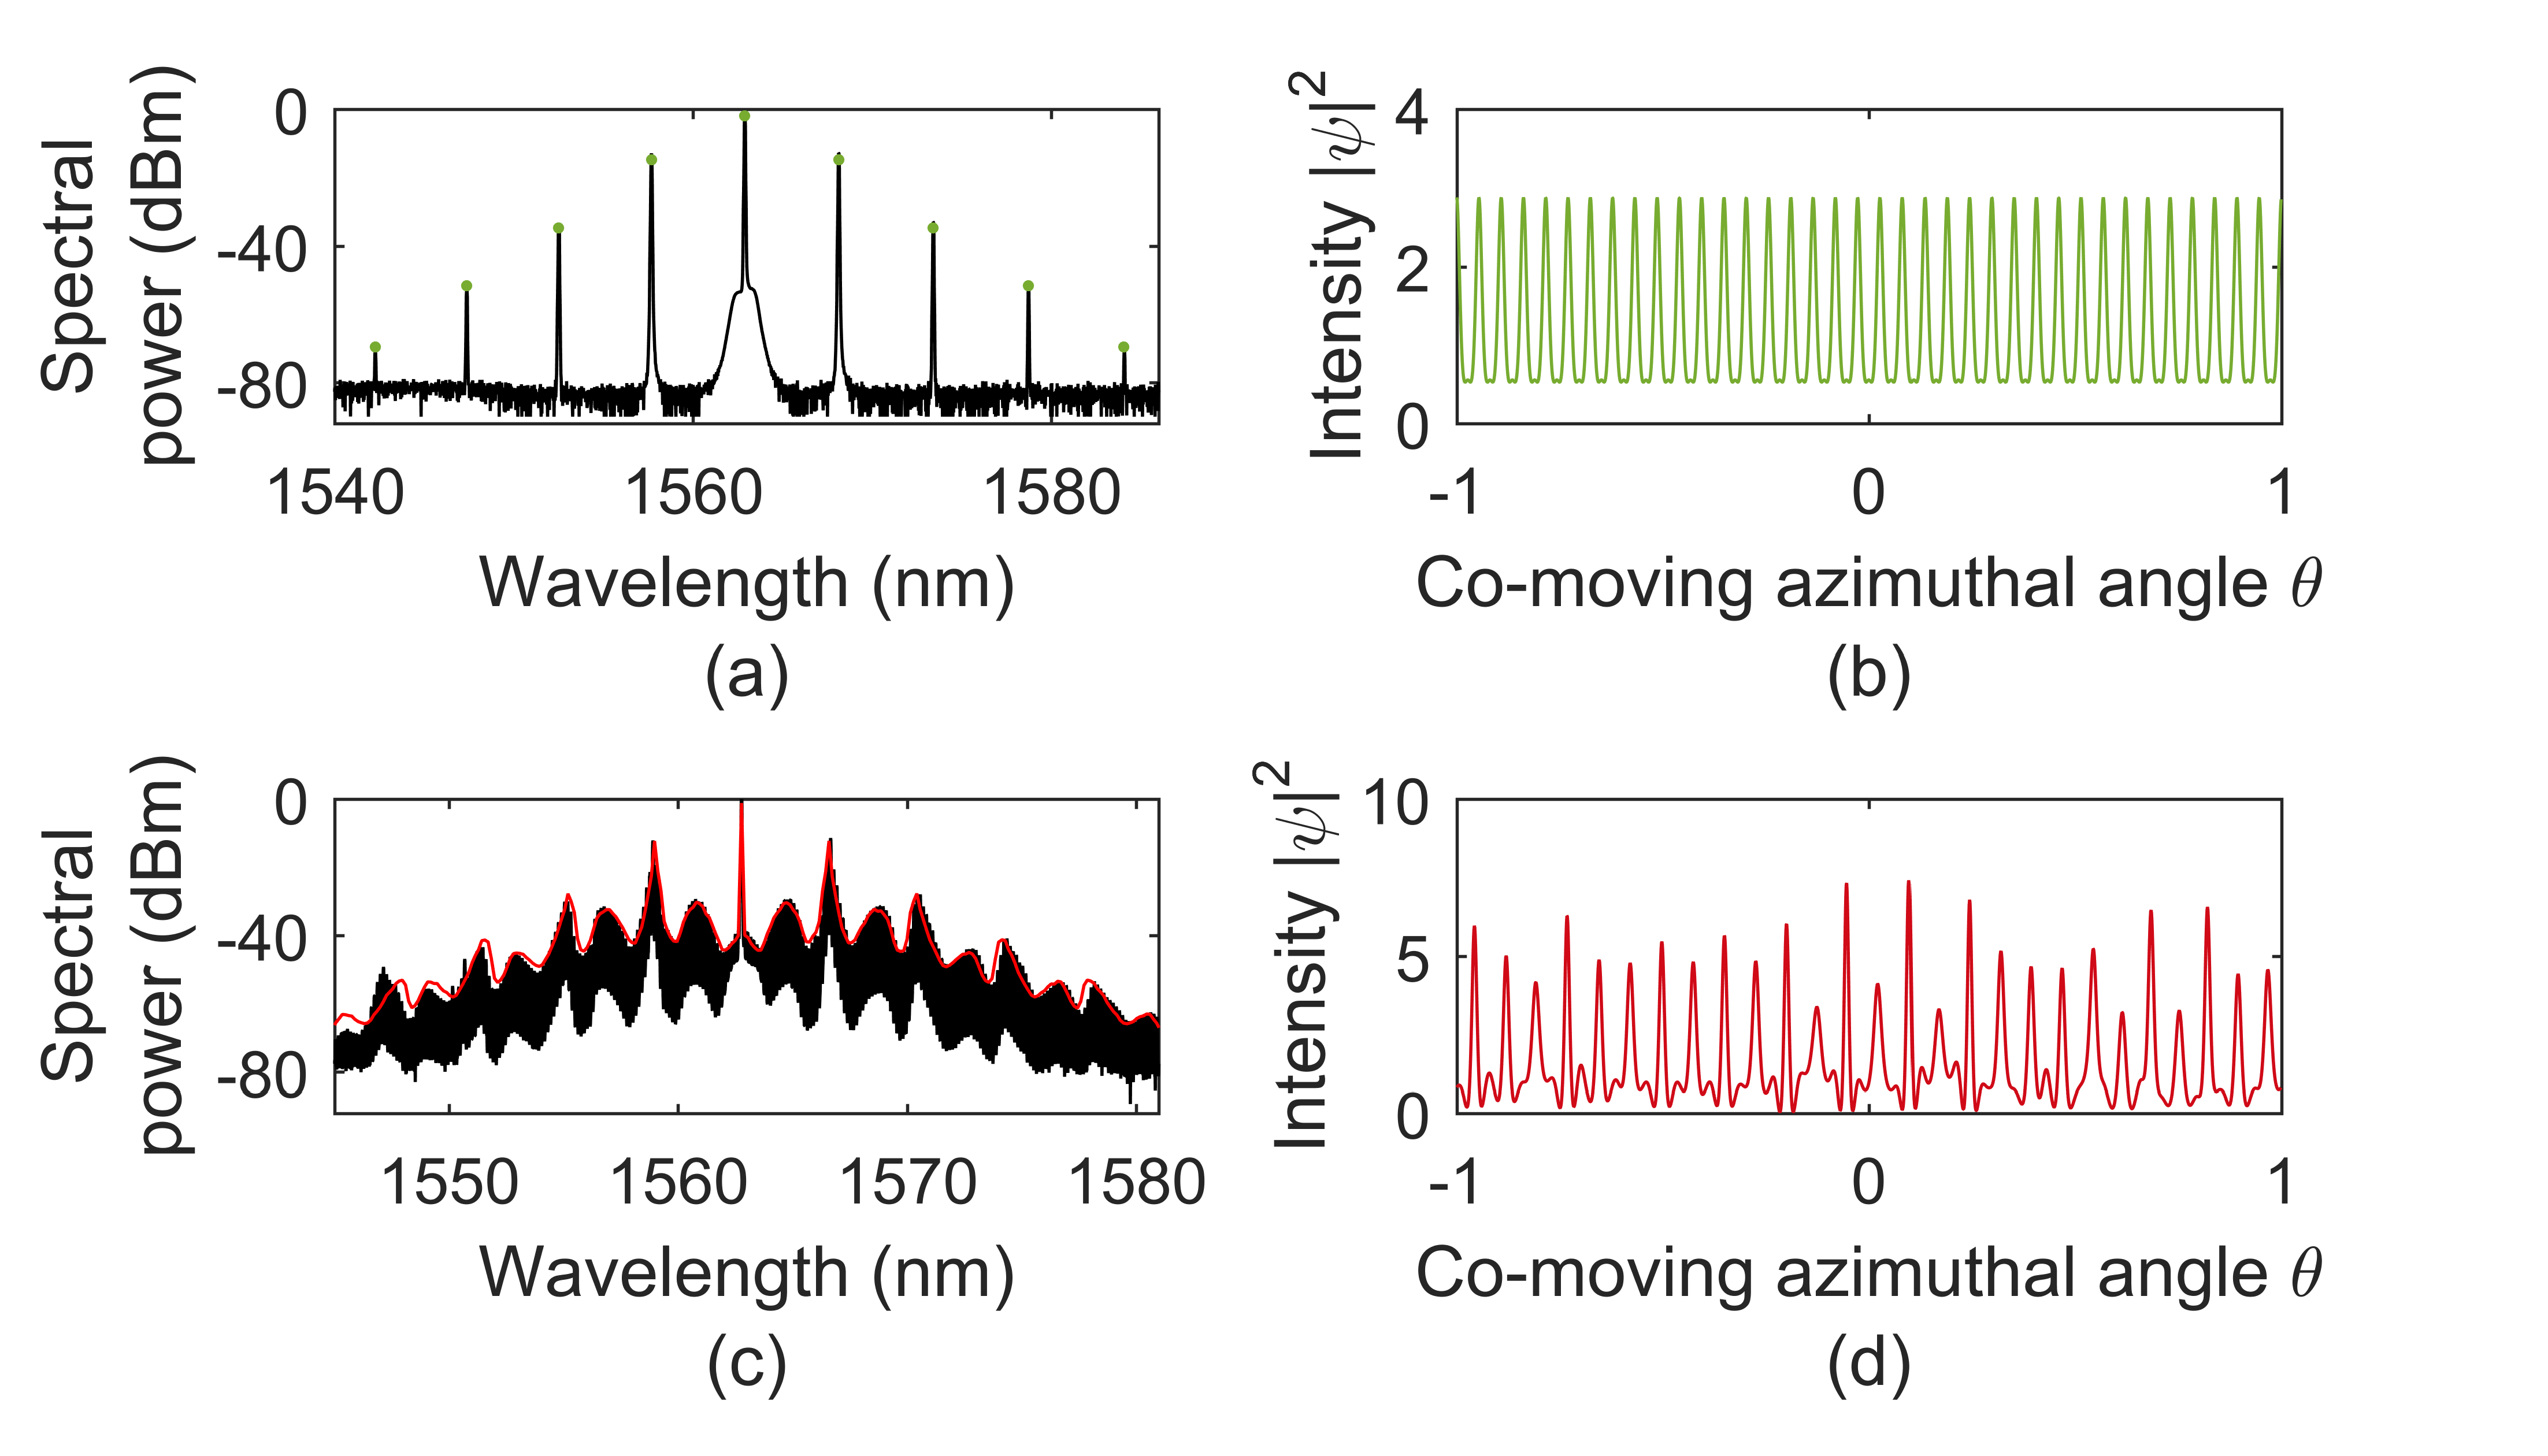
\includegraphics{\FigPath/Figures/Microresonators/MRextendedpatterns.png}
	\end{center}
	\caption[Extended-pattern solutions to the LLE]{\textbf{Extended-pattern solutions to the LLE.} (a,b) Primary-comb pulse train in the frequency (a) and time (b) domains. The primary-comb spectrum corresponds to 39 time-domain pulses. The experimental optical spectrum (black) was obtained in a microdisk resonator with 17.32 GHz free-spectral range, and the simulation (green) is conducted with parameters near typical experimental values: $F^2$=6, $\alpha=-0.6$, and $\beta_2=-0.0044$. (c,d) Spatiotemporal chaos obtained in the same resonator. The experimental measurement (black) yields a time-averaged optical spectrum, with a simulation of qualitatively similar dynamics shown in red. Simulation parameters are $F^2=4.2$, $\alpha=1.2$, and $\beta_2=-0.0054$. A snapshot of the evolving time-domain waveform is shown in (d).
	}
	
	\label{fig:MRextendedpatterns}
\end{figure} 

Relative to generation of solitons, discussed below, experimental generation of an extended pattern is straightforward. These patterns are generated with blue effective pump-laser detuning $\alpha_{eff}<0$, where thermal locking can occur. Because they arise spontaneously from noise, their generation is (comparatively) straightforward: simply decrease the pump-laser frequency until a pattern is generated. Unfortunately, operation of a Kerr-comb in the extended pattern regime is disadvantageous for applications: the $n$-FSR spacing of primary comb presents a challenge for measurement of the repetition rate of the frequency comb due to the bandwidth of measurement electronics and is also an inefficient use of physical space (i.e. for an $n-$pulse primary comb pulse train, an equivalent pulse train can always be obtained using the single-soliton output of a resonator with area that is smaller by a factor of $1/n^2$), and the aperiodic time-evolution of chaotic comb corresponds to modulation sidebands on the comb modes within the linewidth of the cavity that preclude the use of the comb as a set of stable optical reference frequencies. 

An important property of these extended patterns is that they fill the resonator---the characteristic size of temporal features scales roughly as $1/\sqrt{-\beta_2}$, but these features are distributed densely and uniformly throughout the resonator. This means that the total circulating power of an extended pattern $\int d\theta\, |\psi|^2$ is large relative to the localized pulses discussed in the next section, and therefore that extended patterns come with a comparatively large thermal shift of the resonance. As explained below, this contributes to the experimental challenges in soliton generation.



\subsection{Kerr comb outputs: solitons} \label{sec:LLEsolitons}
The term `soliton' generally refers to a localized excitation that can propagate without changing its shape due to a delicate balance between dispersion (or diffraction) and nonlinearity; sometimes known as `solitary waves,' solitons entered the scientific consciousness in the nineteenth century with their observation by John Scott Russell \cite{Russell1844}. They are fundamental solutions to nonlinear partial-differential equations that describe a host of physical phenomena, and are found in several contexts within the field of nonlinear optics: spatial\cite{Lugiato1987,Brambilla1997} and spatiotemporal solitons (light bullets) \cite{Minardi2010} have been studied, and soliton modelocking \cite{Kartner1996,Grelu2012} is an important method of femtosecond pulse generation. Temporal Kerr-soliton pulses in optical fibers are particularly well known \cite{Agrawal2007,Mollenauer2006}, and have been considered as a candidate for fiber-optic communications protocols \cite{Hasegawa1995,Haus1996}. Microresonators support so-called dissipative cavity solitons, which are localized pulses circulating the resonator that are out-coupled once per round trip. In the case of a single circulating soliton, this leads to a train of pulses propagating away from the resonator with repetition rate $1/T_{RT}$. Thus the mode spacing of the comb matches the FSR of the resonator, in contrast with widely-spaced primary comb spectra, and the soliton can, in principle, remain stable and propagate indefinitely as a stationary solution to the LLE. This makes Kerr combs based on solitons particularly attractive for applications.

\subsubsection{Mathematical description of solitons}

Solitons in optical fibers are solutions of the nonlinear Schrodinger equation (NLSE) that describes pulse-propagation in optical fiber \cite{Agrawal2007}:
\begin{equation}
\frac{\partial A}{\partial z}= i\gamma|A|^2 A -i \frac{\beta}{2} \frac{\partial^2 A}{\partial T^2}. \label{NLSE}
\end{equation}
This equation describes the evolution of the pulse envelope $A$ in the `fast-time' reference frame parametrized by $T$ as it propagates down the length of the fiber, parametrized by the distance variable $z$. Here $\gamma=\frac{2\pi}{\lambda}\frac{n_2}{A_{eff}}$ is the nonlinear coefficient of the fiber, where $n_2$ is the Kerr index, $A_{eff}$ is the effective nonlinear mode area and $\lambda$ is the carrier wavelength, and $\beta\equiv\beta_{prop,2}$ is the GVD parameter. The LLE can be viewed as an NLSE with additional loss and detuning terms $-(1+i\alpha)\psi$ and a driving term $F$.

The fundamental soliton solution to the NLSE is:
\begin{equation}
A_{sol}=\sqrt{P_0}\, \mathrm{sech}\left(T/\tau\right)\,e^{i\gamma P_0 z/2+i\phi_0},
\end{equation}
where $P_0$ is the peak power of the pulse and is related to the duration of the pulse $\tau$ via $\tau=\sqrt{-\beta/\gamma P_0}$, and $\phi_0$ is an arbitrary phase. Thus, this equation admits a \textit{continuum} of pulsed fundamental `soliton' solutions, with one existing for each value of the peak power. Each of these solutions propagates down the fiber without changing shape; only the phase evolves with distance as $\phi(z)=\gamma P_0 z/2+\phi_0$.


The introduction of the loss, detuning, and driving terms into the NLSE to obtain the LLE has several important consequences for solitons. First, exact analytical expressions for the soliton solution to the LLE in terms of elementary functions are not known, in contrast with the situation for the NLSE. However, the soliton solutions to the LLE, Eq. \ref{eq:LLE}, can be approximated well as:
\begin{equation}
\psi_{sol}=\psi_{CW,min}+e^{i\phi_0}\sqrt{2\alpha}\,\mathrm{sech}\sqrt{\frac{2\alpha}{-\beta_2}}\theta. \label{eq:LLEsoliton}
\end{equation}
Here $\psi_{CW,min}$ is the flat solution to the LLE from Eq. \ref{eq:LLEflatsoln} at the point where the soliton solution is desired; when multiple flat solutions exist, $\psi_{CW,min}$ is the one corresponding to the smallest intensity $\rho_1$. The phase $\phi_0=\mathrm{cos}^{-1}(\sqrt{8\alpha}/\pi F)$ arises from the intensity-dependent phase shift in the cavity due to the Kerr effect, mathematically described by the term $i|\psi|^2\psi$. We depict this approximation, alongside numerical calculations of exact soliton solutions to the LLE, in Fig. \ref{fig:MRsoliton}.

%\footnote{Perhaps its worth noting that this is a mathematical approximation, in the sense that this is simply a way to approximate the steady-state solution to a differential equation that we don't know how to solve with elementary functions. There isn't any obvious physical approximation we make (e.g. ignoring some particular effect or taking a particular limit) in moving from the exact numerical soliton solution to Eq. \ref{eq:psisol}}

\begin{figure}[htpb]
	\begin{center}
		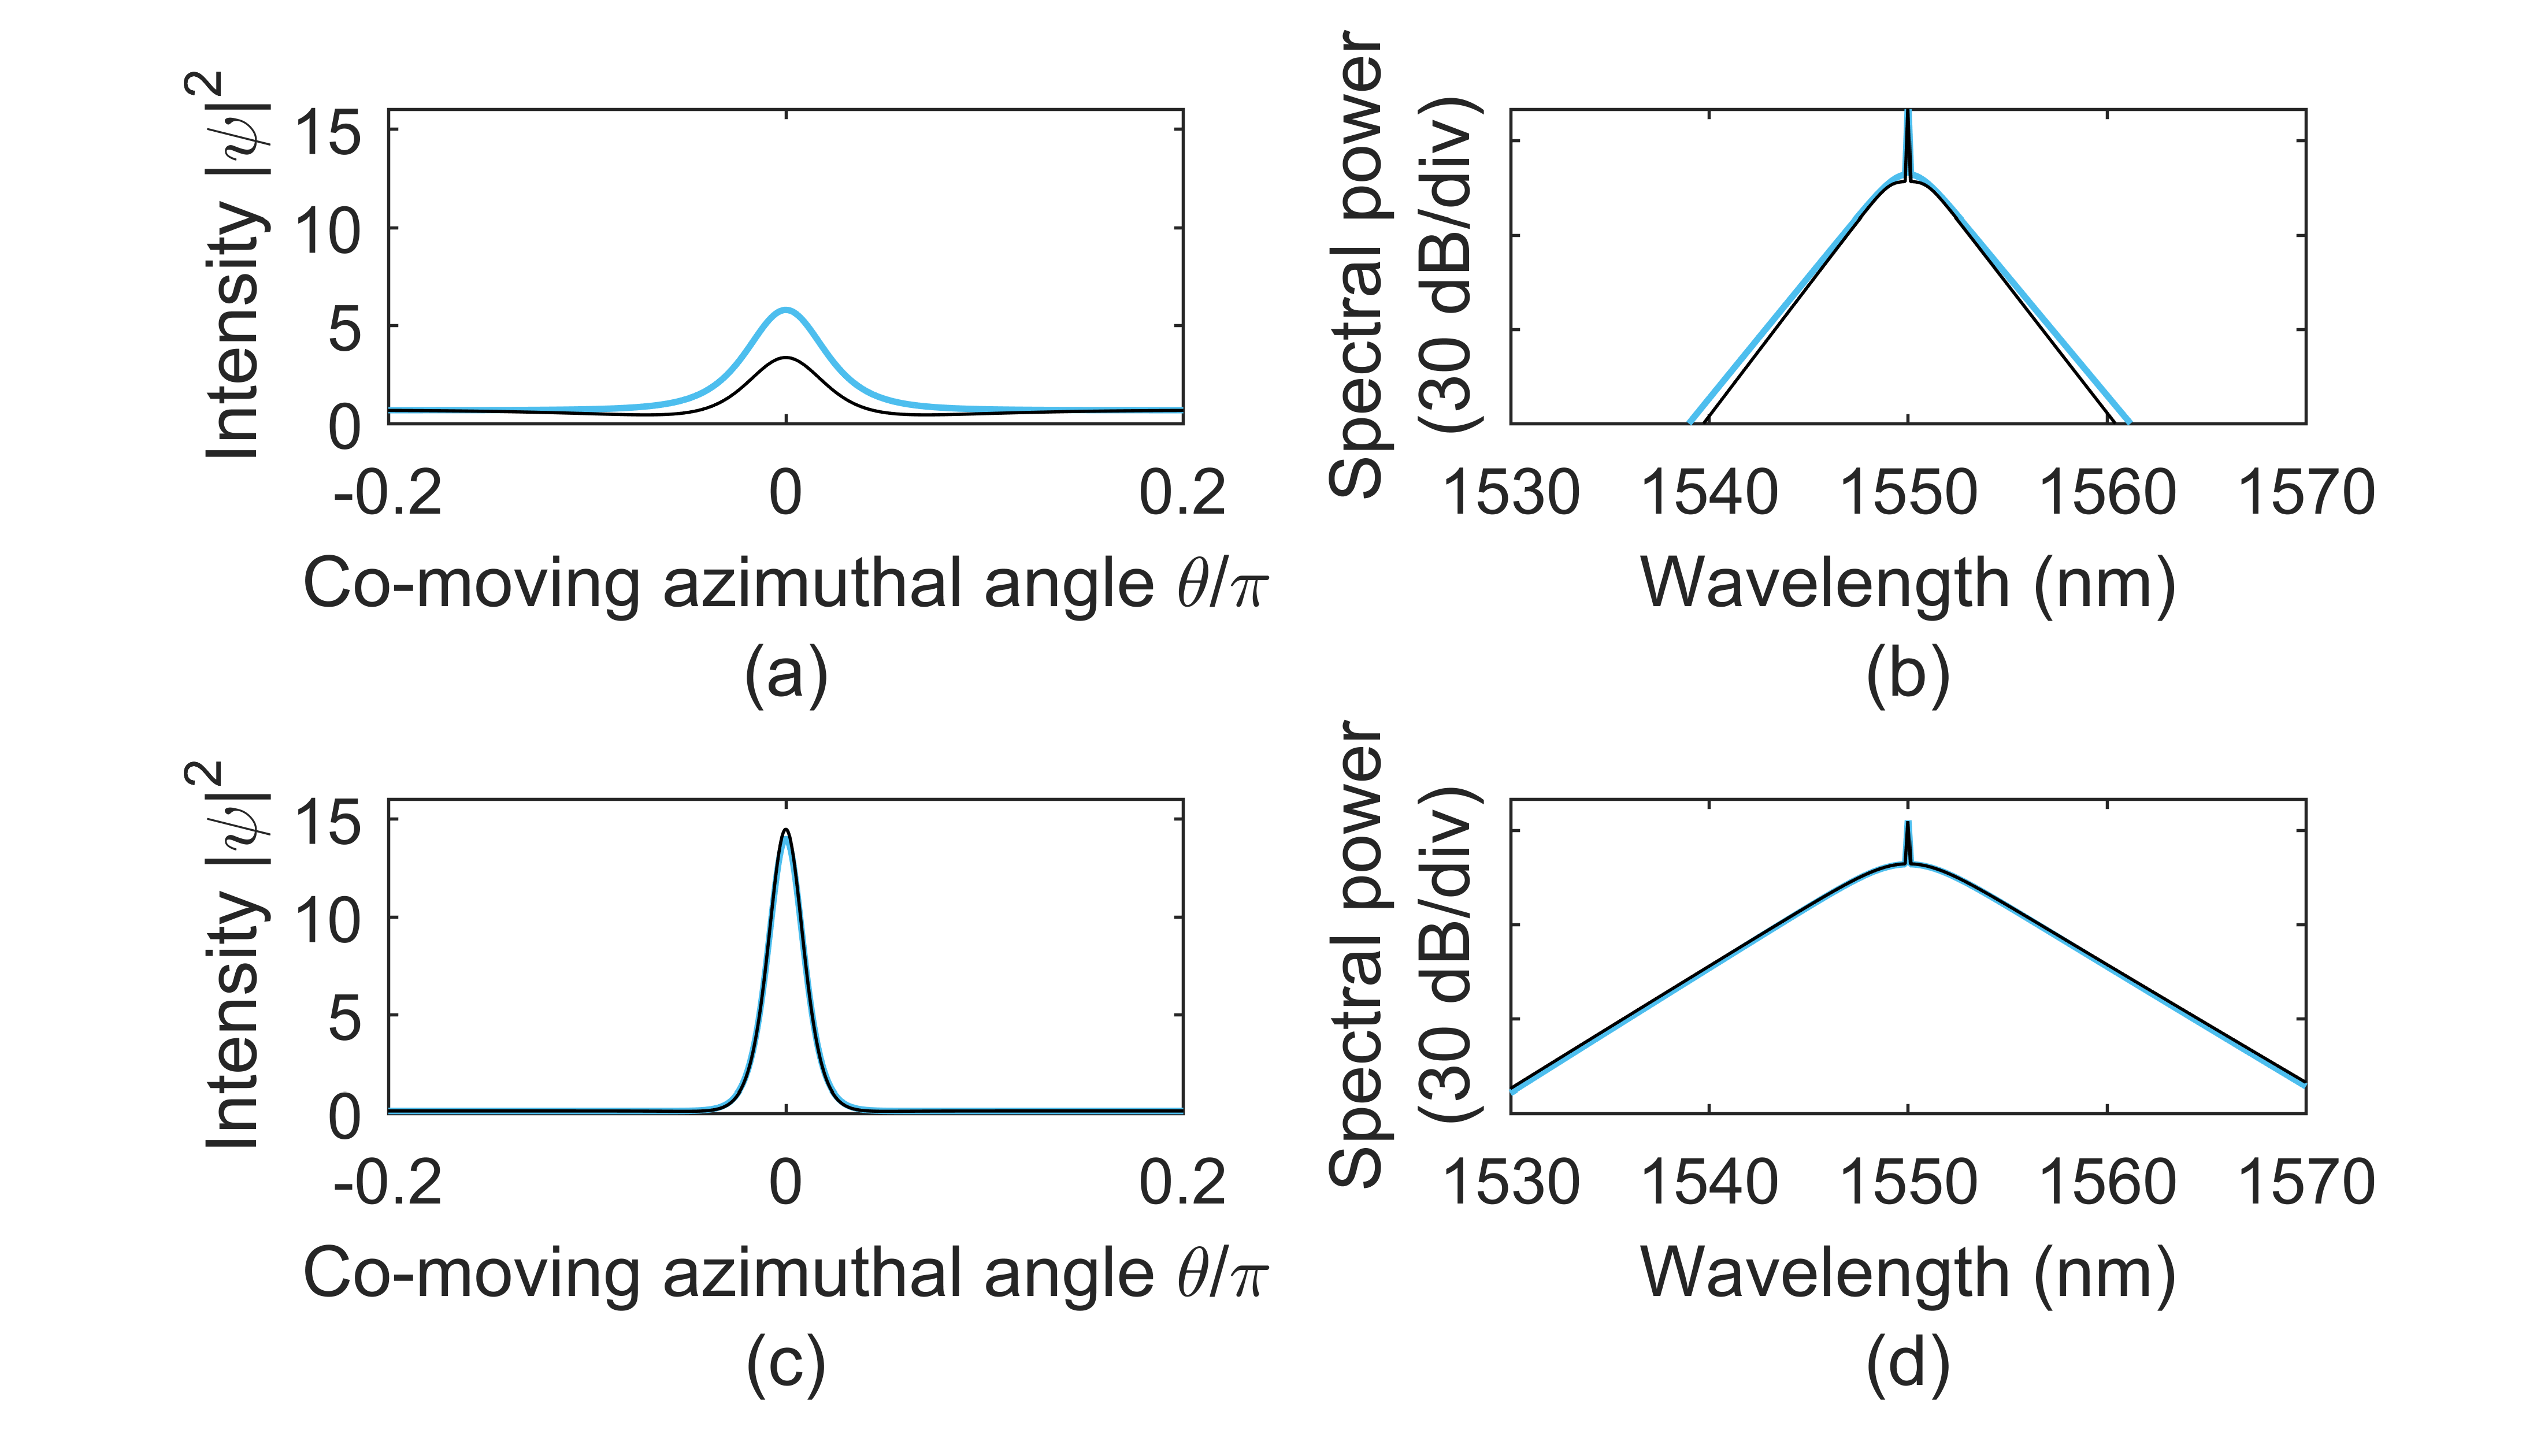
\includegraphics{\FigPath/Figures/Microresonators/MRsoliton.png}
	\end{center}
	\caption[Soliton solutions to the LLE]{\textbf{Soliton solutions to the LLE.} Analytical approximations (color) and numerically-calculated exact solutions (black) to the LLE in the time (a,c) and frequency (b,d) domains. The solitons are calculated at $\alpha=0.95\,\alpha_{max}=0.95\,\pi^2F^2/8$ for $F^2=8\sqrt{3}/9$ (a,b) and $F^2=6$ (c,d) with $\beta_2=-0.02$ in both cases. The isolated spectral spike is at the pump frequency and corresponds to the CW background $\psi_{CW,min}$. Spectra are calculated using $f_{rep}=$16.5 GHz with pump wavelength of $\lambda_p$=1550 nm. For experimental measurements of solitons in microring resonators, see Chapters \ref{chap:SolitonCrystals} and \ref{chap:PMPumping}.
	}
	
	\label{fig:MRsoliton}
\end{figure} 


This approximation $\psi_{sol}$ from Eq. \ref{eq:LLEsoliton} for the soliton solution of the LLE illustrates a second important consequence of the differences between the NLSE and the LLE: while the NLSE admits a continuum of fundamental soliton solutions parametrized by their peak power $P_0$ and arbitrary phase $\phi_0$, the LLE supports only one shape for the envelope of a soliton for fixed experimental parameters.  Intuitively, this can be understood as arising from the need for the round-trip phase shift for all points on the soliton to be zero in steady-state; the introduction of the detuning parameter $\alpha$ breaks the degeneracy that exists for the NLSE within the continuum of soliton solutions.

The analytical approximation in Eq. \ref{eq:LLEsoliton} indicates the scaling of the amplitude and width of the LLE soliton with the experimental parameters: the amplitude of the LLE soliton, prior to its summation with the CW background, depends only on the detuning $\alpha$, and the width of the soliton increases with larger detuning $\alpha$ and smaller dispersion $\beta_2$. Importantly, if one is concerned with maximizing the bandwidth of the soliton, it is important to minimize $\beta_2$ and maximize $\alpha$, due to the inverse relationship between temporal duration and spectral bandwidth. The spectrum of a single-soliton Kerr comb has a $\mathrm{sech}^2\left((\omega-\omega_p)/\Delta \omega_{sol}\right)$ envelope, where $\omega$ is the optical angular frequency and $\Delta\omega_{sol}\approx\sqrt{32\alpha/|\beta_2| T_{RT}^2 }$ is the bandwidth of the pulse in angular frequency. Equivalently, the bandwidth of the soliton in (linear) optical frequency is $\sqrt{\frac{16\Delta\nu f_{rep}^2}{D_2}\alpha}$, where $\Delta\nu$ is the resonance linewidth in linear frequency; the spectral width in mode number is $\Delta\mu_{sol}\approx4\sqrt{\alpha\Delta\nu/D_2}$. Consistent with the phase $\phi_0$ in the approximation $\psi_{sol}$ in Eq. \ref{eq:LLEsoliton}, solitons can exist up to a maximum detuning of $\alpha_{max}\sim\pi^2 F^2/8$ \cite{Herr2014}. For a soliton at the maximum detuning for fixed normalized pump power $F^2$, the bandwidth is then $\sqrt{\frac{\pi^2\Delta\nu f_{rep}^2}{2 D_2}F^2}$. 

Solitons exist only where there is a stable flat solution $\psi_{CW}$ that is effectively red detuned that can form the background for the pulse \cite{Barashenkov1996,Coen2013}. This effectively red-detuned background is itself thermally unstable (see Sec. \ref{sec:thermaleffects}), but the existence of the soliton acts to stabilize the pump detuning. As explained by Herr et al., the soliton provides a local modulation of the refractive index through the Kerr effect, which changes the round-trip phase shift of pump light that arrives coincidentally with the soliton at the coupling port \cite{Herr2014}. This leads to a \textit{local} increase in the resonant wavelength for this pump light. Thus there are effectively two resonant wavelengths, a smaller one determined by the round-trip phase shift including the Kerr shift from the CW background, and a larger one determined by the round-trip phase shift including the Kerr shift from the soliton \cite{Guo2017a}. The pump laser can be effectively blue-detuned with respect to the latter resonance, which can lead to thermally stable operation in the soliton regime.

%is clearly valid only for red pump-laser detuning  Solitons exist as solutions to the LLE only for red pump-laser detuning $\alpha>0$.

Solitons are strongly localized: as can be seen from Eq. \ref{eq:LLEsoliton}, the deviation of the background intensity from $\rho_1$ near a soliton at $\theta_0$ is proportional to $e^{-(\theta-\theta_0)/\delta\theta}$, where $\delta\theta=\sqrt{-\beta_2/2\alpha}$. If $\delta\theta$ is sufficiently small, multiple solitons can be supported in the resonator domain $-\pi\leq\theta\leq\pi$ with very weak interactions between solitons. If the separation between solitons $i$ and $j$ at $\theta_i$ and $\theta_j$ is small relative to $\delta\theta$, the solitons will interact. The topic of soliton interactions is complicated in general, with different types of interactions in different systems (see e.g. Refs. \cite{Zabusky1965,Gordon1983,Malomed1991,Jang2013}). Simulations reveal that if $(\theta_i-\theta_j)/\delta\theta$ is too small, LLE solitons exhibit attractive interactions as a result of the monotonic (as opposed to oscillatory) decay of the localized pulse to $\psi_{CW}$ \cite{Parra-Rivas2017}, which precludes the existence of stable equilibrium separations. The result of this attraction can be pair-wise annihilation or merger, with the ultimate result being an ensemble with fewer solitons. The maximum number of solitons that can coexist in a resonator in the absence of higher-order stabilizing effects (see Chapter \ref{chap:SolitonCrystals} and Refs. \cite{Wang2017,Parra-Rivas2017}) can be approximated as $N_{max}\approx\sqrt{-2/\beta_2}$ \cite{Herr2014}. An approximation to the form of a soliton ensemble is possible as:

\begin{equation}
\psi_{ens}=\psi_{CW,min}+e^{i\phi_0}\sqrt{2\alpha}\sum_j \mathrm{sech}\left(\sqrt{\frac{2\alpha}{-\beta_2}}(\theta-\theta_j)\right),\label{eq:LLEsolens}
\end{equation}
where $\{\theta_j\}$ define the positions of the solitons in the ensemble and $\phi_0=\mathrm{cos}^{-1}(\sqrt{8\alpha}/\pi F)$ as above. Fig. \ref{fig:MRenergylevels} provides an example illustrating the degeneracy in soliton number of Kerr-combs operating in the soliton regime.

\begin{figure}[htpb]
	\begin{center}
		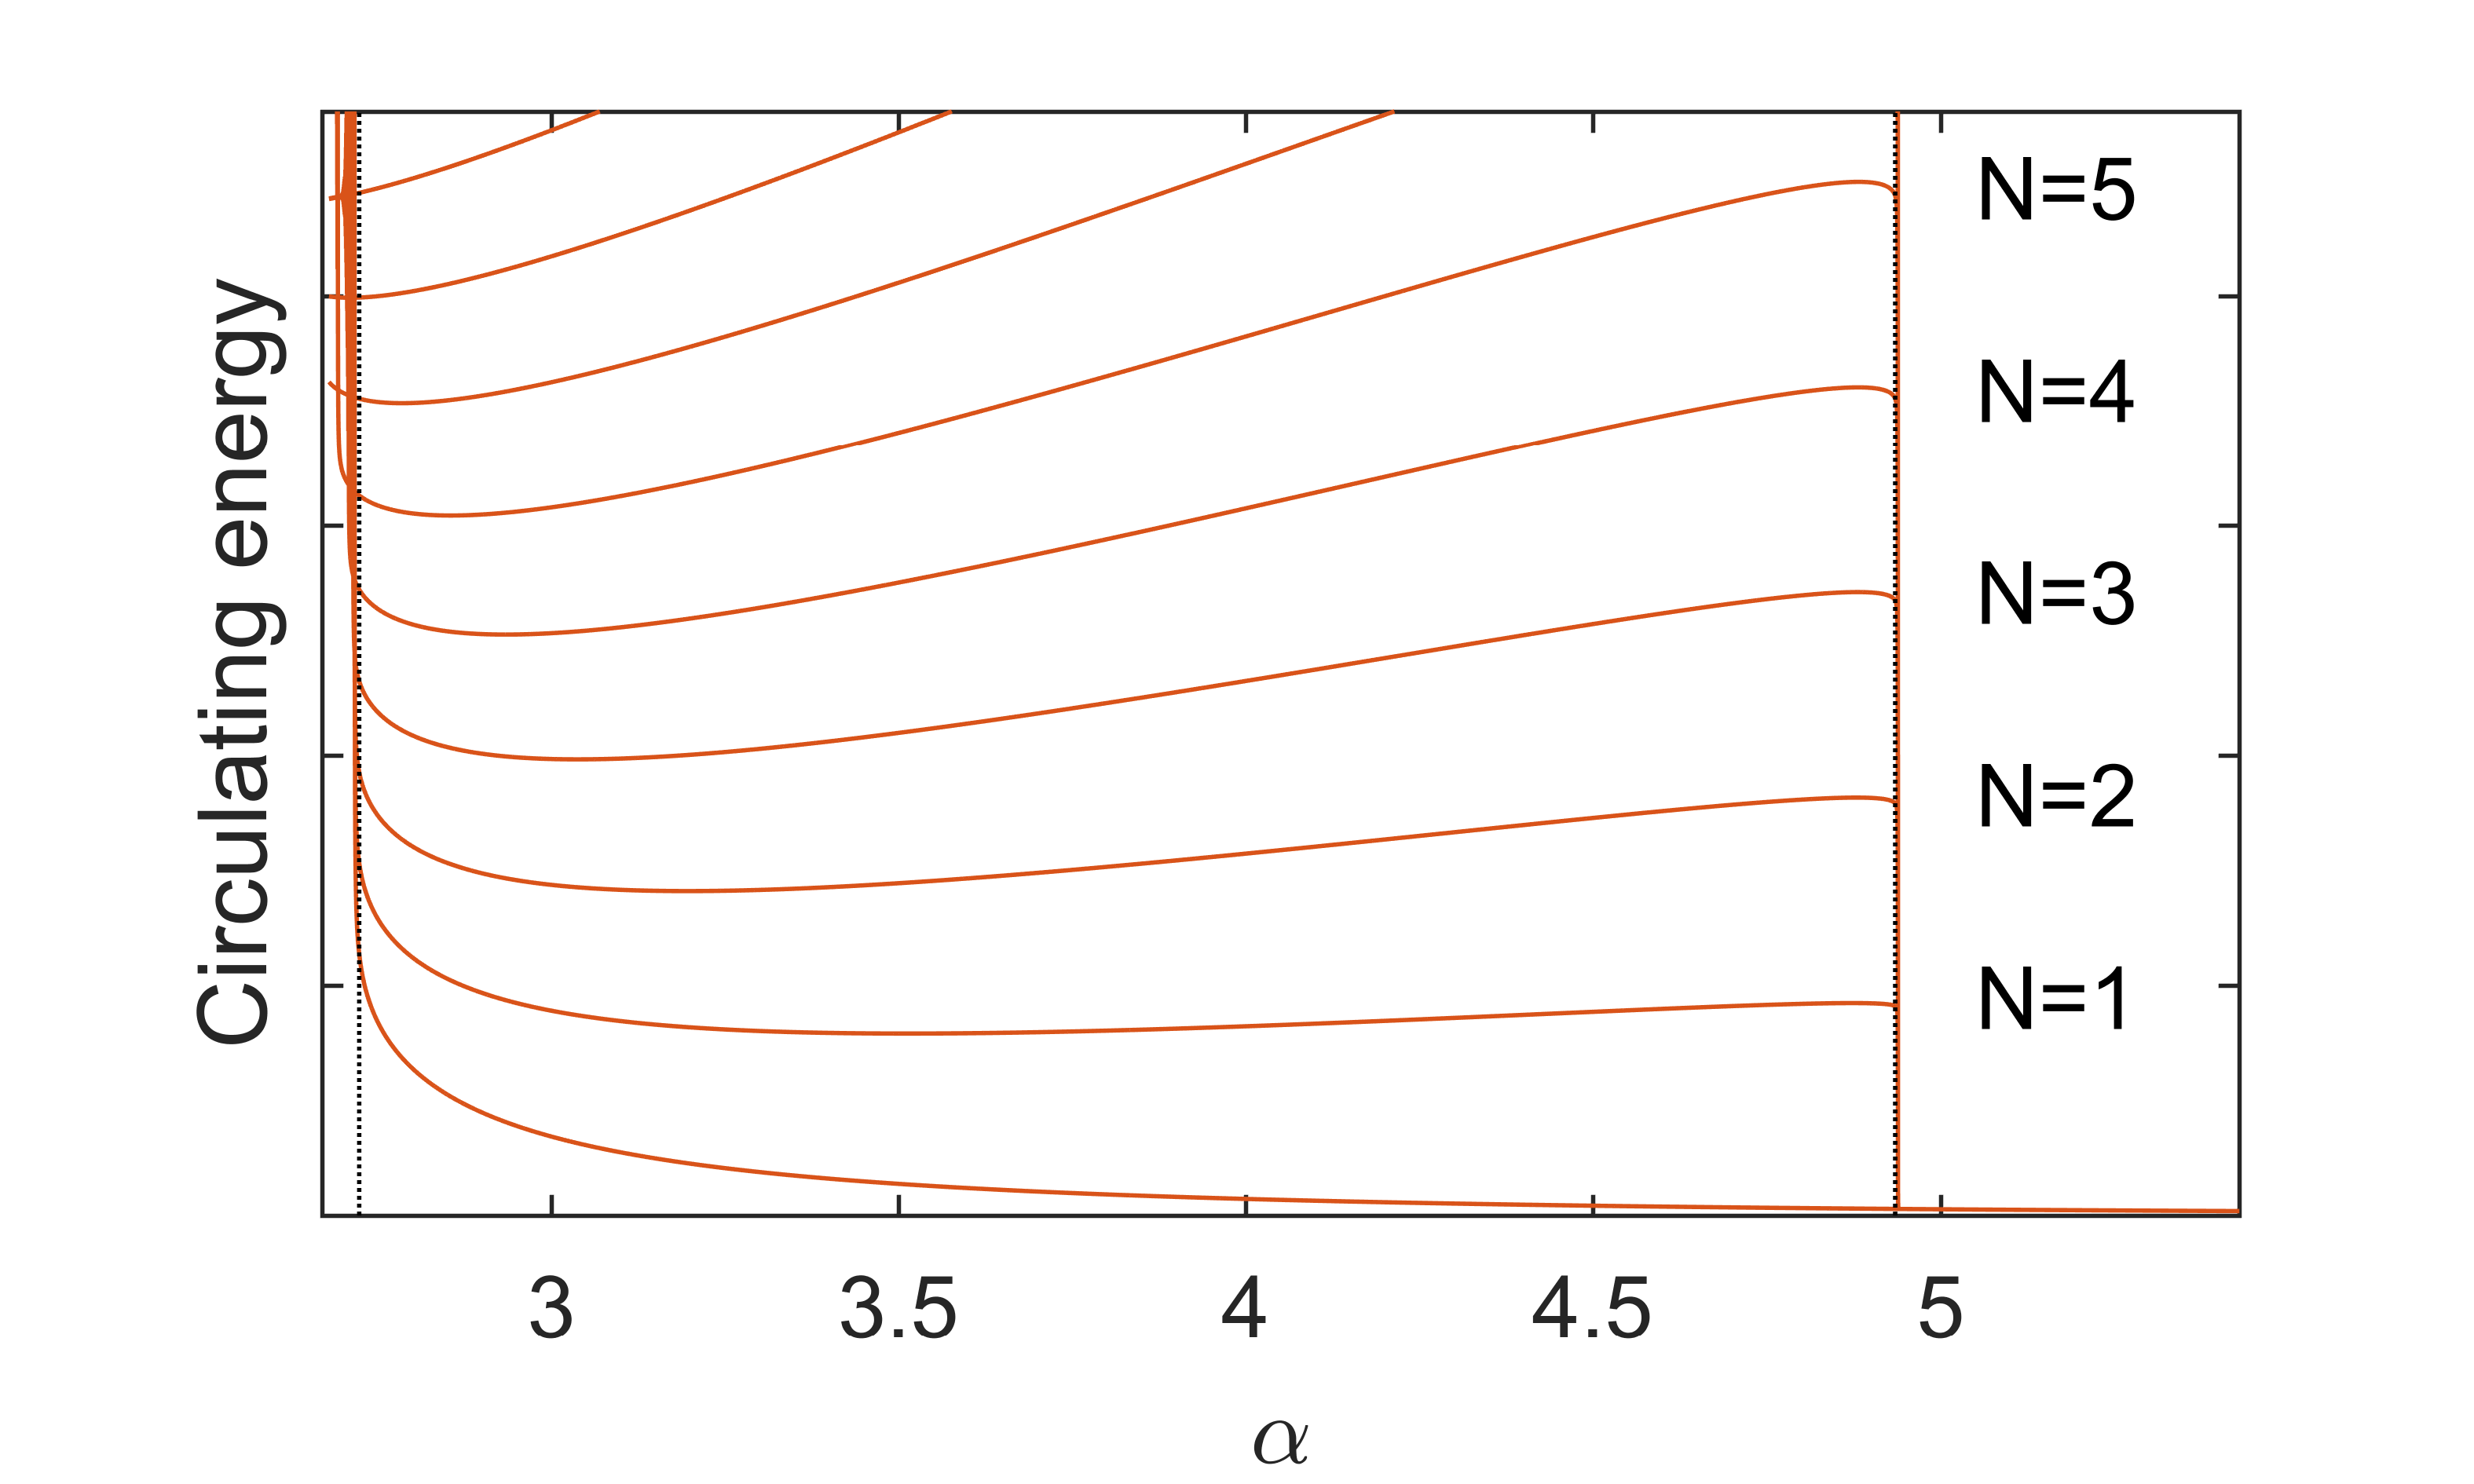
\includegraphics{\FigPath/Figures/Microresonators/MRenergylevels_slower.png}
	\end{center}
	\caption[Kerr-soliton energy-level diagram]{\textbf{Kerr-soliton energy-level diagram.} Some of the possible values of the circulating energy (proportional to $\int d\theta\,|\psi|^2$) in the soliton regime as a function of the detuning parameter $\alpha$. Level curves correspond to the number of circulating solitons. This diagram is obtained from numerical solutions using $F^2=4$, $\beta_2=-0.0187$, and is quantitatively dependent on both of these parameters. Dotted vertical lines indicate approximations to the minimum and maximum detunings for solitons. The approximation for the minimum detuning is the value of $\alpha$ at which the effectively red-detuned branch vanishes, obtained by inserting $\rho_-$ (Eq. \ref{eq:rhopm}) into Eq. \ref{eq:LLEstat2} for $F^2=4$ and solving for $\alpha$, and the approximate maximum detuning is $\alpha_{max}=\pi^2 F^2/8$.}
	
	\label{fig:MRenergylevels}
\end{figure} 
%A single soliton is a localized pulse that is repeated once each round-trip; therefore a single soliton is a single-FSR frequency comb, in contrast with the primary comb output discussed above. 





\subsubsection{Microresonator solitons in experiments}


Relative to the generation of extended modulation-instability patterns, experimental generation of solitons in microring resonators is challenging. Solitons are localized excitations below threshold, which means that their existence is degenerate with their absence---a resonator can host $N=0, 1, 2,...$ up to $N_{max}$ solitons for a given set of parameters $\alpha$ and $F^2$; as discussed above and illustrated in Fig. \ref{fig:MRenergylevels}. If $\alpha$ and $F^2$ are experimentally tuned to a point at which solitons may exist, $\psi$ will evolve to a form determined by the initial conditions of the field $\psi_0$. To provide initial conditions that evolve to $N>0$ solitons, most experimental demonstrations of soliton generation have involved first generating an extended pattern in the resonator, and then tuning to an appropriate point $(\alpha,F^2)$ so that `condensation' of solitons from the extended pattern occurs. 

Condensation of solitons from an extended pattern presents additional challenges. First, it is difficult to control the number of solitons that emerge, due to the high degree of soliton-number degeneracy as shown in Fig. \ref{fig:MRenergylevels}. This typically leads to a success rate somewhat lower than 100 $\%$ in the generation of single solitons. Second, the transition from a high duty-cycle extended pattern to a lower duty-cycle ensemble of one or several solitons comes with a dramatic drop in intracavity power that occurs on the timescale of the photon lifetime. If the resonator is in thermal steady-state before this drop occurs, the resonator will cool and the resonance frequency will increase. If this increase is large enough that the final detuning $\alpha$ exceeds $\alpha_{max}=\pi^2 F^2/8$, the soliton is lost. This challenge can be addressed by preparing initial conditions for soliton generation and then tuning to an appropriate point $(\alpha,F^2$) faster than the cavity can come into thermal steady-state at the temperature determined by the larger power of the extended pattern; this is possible because the timescale over which an extended pattern can be generated is related to the photon lifetime, which is typically much faster than the thermal timescale.

The first report of soliton generation in microresonators came in 2012 in a paper by Herr et al. \cite{Herr2014} (2012 pre-print \cite{Herr2012a}). These authors described optimizing the speed of a decreasing-frequency scan of the pump laser across the cavity resonance so that solitons could be condensed from an extended pattern and the scan could then be halted at a laser frequency where the solitons could be maintained with the system in thermal steady-state at the temperature determined by the circulating power of the solitons. Stochastic reduction in the number of solitons in the resonator after condensation from an extended pattern was identified in these experiments. This corresponds to transitions between levels in the diagram in Fig. \ref{fig:MRenergylevels}, and is associated with discrete steps in a measurement of the `comb power,' the output power of the resonator with the pump frequency $\nu_p$ filtered out. The resulting staircase-like nature of a comb power measurement is a useful experimental signature of soliton generation in microresonators, and is important for comparison with the results described in Chapter \ref{chap:PMPumping}.

%The results of a simulation of these dynamics are shown in Fig. \ref{fig:MRsteps}; the staircase-like nature of the end of the scan is a useful experimental signature of soliton generation in microresonators and is important for comparison with the results described in Chapter \ref{chap:PMpumping}.

Other approaches for dealing with the challenges described above have been developed since this first demonstration; these include fast manipulation of the pump power \cite{Brasch2016,Yi2015} or frequency \cite{Stone2017}, periodic modulation of the pump laser's phase or power at $f_{FSR}$ \cite{Lobanov2016,Obrzud2017}, tuning of the cavity resonance frequency using chip-integrated heaters instead of tuning the pump-laser frequency \cite{Joshi2016a,Wang2018a}, and soliton-ensemble preparation and subsequent population reduction through manipulation of the pump laser \cite{Guo2017a}. These methods continue to make use of extended patterns to provide initial conditions for soliton generation. In formally-equivalent fiber-ring resonators, direct generation of solitons without condensation from an extended pattern has been demonstrated using transient phase and/or amplitude modulation of the pump laser \cite{Jang2015,Jang2015a,Wang2018}. 

%Chapter \ref{chap:PMpumping} of this thesis presents a new variation on these schemes that enables direct generation of solitons using only phase modulation at $f_{FSR}$ without transient manipulation of the system parameters; this approach is based on a proposal by Taheri, Eftekhar, and Adibi \cite{Taheri2015}. 

\subsubsection{Microresonator solitons in applications}

Because solitons have single-FSR spacing, have the output localized into a high peak-power pulse, and are stationary (in contrast with chaos, which has single-FSR spacing but is not stationary), they are promising for applications. Many of the proposals for and demonstrations of applications with Kerr-combs have used single-soliton operation. Some of the applications already demonstrated include an optical clock \cite{Papp2014}, dual-comb spectroscopy \cite{Suh2016a}, coherent communications \cite{Marin-Palomo2017}, and direct on-chip optical frequency synthesis \cite{Spencer2018}. Additionally, soliton combs have been self-referenced both with \cite{Jost2015,DelHaye2016} and without \cite{Brasch2017,Briles2017} external spectral broadening. Nevertheless, there remains work to be done to bring microresonator-soliton technology to the level of maturity that will be required for deployment in the field. Chapters \ref{chap:PMPumping} and \ref{chap:SolitonCrystals} describe two recent advancements: the development of a method for direct on-demand generation of single solitons by use of a phase-modulated pump laser, and the observation and explanation of a soliton-interaction mechanism that imparts rigid structure on the allowed configurations of multi-soliton ensembles.



%\section{Frequency comb nonlinear dynamics in microresonators}
%
%The first report of frequency-comb generation in silica microcavities by Del'Haye et al initiated a serious research effort to understand how to make these combs useful for applications. The early years of this effort brought reports of comb generation in resonators made from amorphous \cite{stuff} and crystalline \cite{stuff} materials, with 



%
%
%
%
%
%
%that exhibit the  nonlinearity, which can be the dominant source of nonlinearity in centro-symmetric materials in which the second-order nonlinearity $\chi{(2)}$ must vanish. The $\chi^{(3)}$ nonlinearity, or Kerr nonlinearity, arises from the term in the Taylor expansion for the polarization response of the medium that scales with the optical intensity: $P_{NL}=...+\epsilon_0 \chi^{(3)} E^3+...$. \cite{something}. This can equivalently and usefully be described as a dependence of the refractive index on the intensity via .
%
%The third-order 
%
%The resonator quality factor is an important figure of merit for the use of optical resonators as platforms for nonlinear optics. This is discussed extensively below; typically the threshold power for nonlinear optics scales as $Q^{-2}$, meaning that in the design of practical platforms targeting high $Q$ is an important consideration. Fabrication of ultrahigh-Q resonators has been achieved with a variety of designs and materials, including ... 
%
%
% These resonators can be constructed with extremely high quality factors, upwards of $10^8$, which facilitates high circulating intensity. 
% 
% Combs using optical ring resonators leverage this confinement and the resulting long photon lifetimes in high-quali oty factor resonators 